\section{Chapter 2}

\begin{table}[ht]
\centering
\begin{tabular}{lrrr}
  \toprule
Gene set name & n genes & $\beta$ & p \\ 
  \midrule
Exocytosis & 83 & 0.19 & 0.039 \\ 
  Neurotransmitter metabolism & 27 & -0.10 & 0.686 \\ 
  Excitability & 57 & 0.38 & 0.005 \\ 
  Protein cluster & 43 & 0.20 & 0.091 \\ 
  Ligand-gated ion channel signaling & 33 & 0.03 & 0.438 \\ 
  Tyrosine kinase signaling & 7 & 0.22 & 0.308 \\ 
  Unassigned & 59 & 0.07 & 0.301 \\ 
  Peptide/neurotrophin signals & 28 & 0.04 & 0.430 \\ 
  Intracellular signal transduction & 148 & -0.04 & 0.697 \\ 
  Ion balance/transport & 41 & -0.01 & 0.522 \\ 
  G-protein relay & 27 & -0.10 & 0.688 \\ 
  RNA and protein synthesis, folding and breakdown & 67 & 0.01 & 0.448 \\ 
  Endocytosis & 25 & -0.17 & 0.804 \\ 
  Structural plasticity & 95 & -0.06 & 0.731 \\ 
  Cell metabolism & 51 & -0.13 & 0.827 \\ 
  Cell adhesion and trans-synaptic signaling & 76 & 0.29 & 0.009 \\ 
  G-protein-coupled receptor signaling & 41 & 0.09 & 0.300 \\ 
  Intracellular trafficking & 75 & 0.04 & 0.344 \\ 
   \bottomrule
\end{tabular}
\caption{Synaptic enrichment using components. Intelligence Discovery} \tiny\url{source('~/RProjects/redo_chapter2/R/redo_synapse_set_int_curated.R')} 
\label{tab:MAGMA enrichment of synaptic groups UKBBint}
\end{table}

% latex table generated in R 3.6.3 by xtable 1.8-4 package
% Sun Aug  9 12:41:54 2020
\begin{table}[ht]
\centering
\begin{tabular}{lrrr}
   \toprule
Gene set name & n genes & $\beta$ & p\\
  \midrule
Exocytosis & 83 & 0.04 & 0.348 \\ 
  Neurotransmitter metabolism & 27 & -0.08 & 0.648 \\ 
  Excitability & 57 & 0.43 & 0.003 \\ 
  Protein cluster & 43 & -0.14 & 0.813 \\ 
  Ligand-gated ion channel signaling & 33 & 0.18 & 0.178 \\ 
  Tyrosine kinase signaling & 7 & -0.18 & 0.658 \\ 
  Unassigned & 59 & 0.08 & 0.276 \\ 
  Peptide/neurotrophin signals & 28 & -0.20 & 0.828 \\ 
  Intracellular signal transduction & 148 & 0.07 & 0.226 \\ 
  Ion balance/transport & 41 & 0.11 & 0.242 \\ 
  G-protein relay & 27 & -0.09 & 0.671 \\ 
  RNA and protein synthesis, folding and breakdown & 67 & 0.10 & 0.198 \\ 
  Endocytosis & 25 & 0.12 & 0.281 \\ 
  Structural plasticity & 95 & 0.04 & 0.355 \\ 
  Cell metabolism & 51 & 0.05 & 0.374 \\ 
  Cell adhesion and trans-synaptic signaling & 76 & 0.39 & 0.001 \\ 
  G-protein-coupled receptor signaling & 41 & -0.01 & 0.517 \\ 
  Intracellular trafficking & 75 & -0.06 & 0.713 \\ 
   \hline
   \bottomrule
\end{tabular}
\caption{Synaptic enrichment using components. Education Discovery } 
\label{tab:MAGMA enrichment of synaptic groups UKBBEd}
\end{table}

% latex table generated in R 3.6.3 by xtable 1.8-4 package
% Sun Aug  9 12:43:33 2020
\begin{table}[ht]
\centering
\begin{tabular}{lrrr}
  \toprule 
Gene set name & n genes & $\beta$ & p\\
  \midrule
Cell adhesion and trans-synaptic signaling & 76 & 0.11 & 0.155 \\ 
  Cell metabolism & 51 & -0.07 & 0.726 \\ 
  Endocytosis & 25 & -0.03 & 0.572 \\ 
  Excitability & 57 & 0.13 & 0.159 \\ 
  Exocytosis & 83 & 0.18 & 0.016 \\ 
  G-protein-coupled receptor signaling & 41 & 0.15 & 0.162 \\ 
  G-protein relay & 27 & 0.11 & 0.251 \\ 
  Intracellular signal transduction & 148 & 0.07 & 0.150 \\ 
  Intracellular trafficking & 75 & -0.01 & 0.522 \\ 
  Ion balance/transport & 41 & -0.17 & 0.898 \\ 
  Ligand-gated ion channel signaling & 33 & -0.27 & 0.944 \\ 
  Neurotransmitter metabolism & 27 & 0.25 & 0.099 \\ 
  Peptide/neurotrophin signals & 28 & -0.10 & 0.720 \\ 
  Protein cluster & 43 & 0.11 & 0.207 \\ 
  RNA and protein synthesis, folding and breakdown & 67 & 0.11 & 0.120 \\ 
  Structural plasticity & 95 & -0.10 & 0.874 \\ 
  Tyrosine kinase signaling & 7 & -0.45 & 0.880 \\ 
  Unassigned & 58 & -0.03 & 0.620 \\ 
   \bottomrule
\end{tabular}
\caption{Synaptic enrichment using component Intelligence Discovery sample} 
\label{tab:MAGMA enrichment of synaptic groups ctg}
\end{table}

% latex table generated in R 3.6.3 by xtable 1.8-4 package
% Sun Aug  9 12:45:12 2020
\begin{table}[ht]
\centering
\begin{tabular}{lrrr}
  \toprule
Gene set name & n genes & $\beta$ & p\\
  \midrule
Cell adhesion and trans-synaptic signaling & 76 & 0.17 & 0.067 \\ 
  Cell metabolism & 53 & -0.02 & 0.549 \\ 
  Endocytosis & 26 & 0.11 & 0.251 \\ 
  Excitability & 57 & 0.16 & 0.122 \\ 
  Exocytosis & 83 & -0.11 & 0.877 \\ 
  G-protein-coupled receptor signaling & 41 & 0.08 & 0.315 \\ 
  G-protein relay & 27 & -0.01 & 0.521 \\ 
   Intracellular signal transduction & 147 & 0.02 & 0.418 \\ 
  Intracellular trafficking & 75 & -0.02 & 0.590 \\ 
  Ion balance/transport & 40 & 0.05 & 0.370 \\ 
  Ligand-gated ion channel signaling & 33 & 0.18 & 0.158 \\ 
  Neurotransmitter metabolism & 27 & -0.15 & 0.774 \\ 
  Peptide/neurotrophin signals & 28 & 0.11 & 0.267 \\ 
  Protein cluster & 42 & -0.20 & 0.910 \\ 
  RNA and protein synthesis, folding and breakdown & 66 & 0.22 & 0.016 \\ 
  Structural plasticity & 95 & 0.10 & 0.140 \\ 
  Tyrosine kinase signaling & 7 & -0.27 & 0.742 \\ 
  Unassigned & 58 & 0.07 & 0.290 \\ 
   \bottomrule
\end{tabular}
\caption{Synaptic enrichment using components. Educational attainment replication } 
\label{tab:MAGMA enrichment of synaptic groups EA2}
\end{table}
\clearpage
\begin{figure}
    \centering
    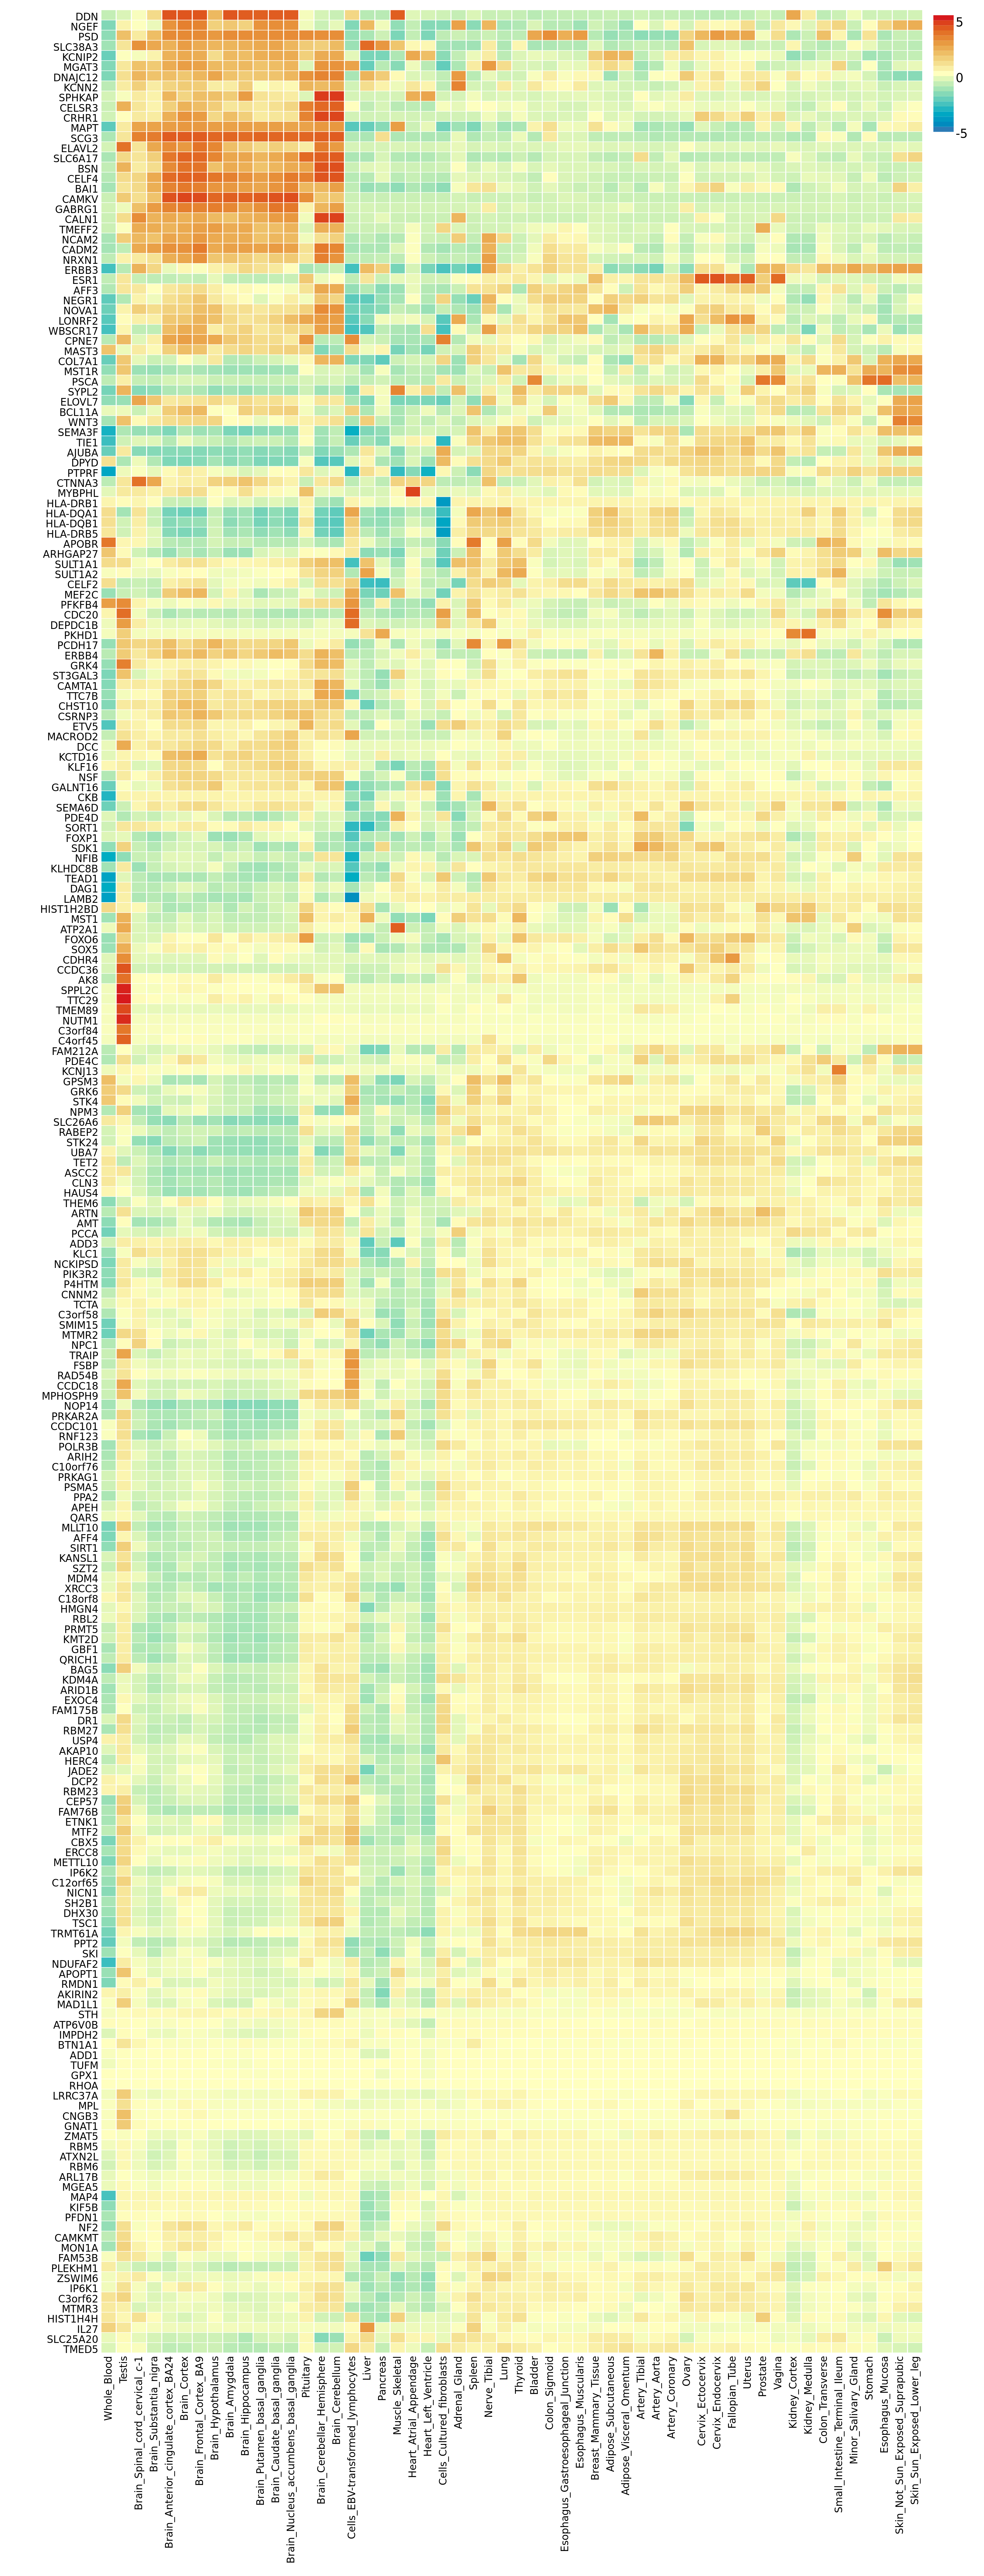
\includegraphics[height=25cm]{images/FUMA_plots/expHeat_FUMA_gene2func-2_ukbbed_zeromean.png}
    \caption{Heatmap gene expression FUMA UKBBEd Average value of the relavitve expression level zero mean centred and log2 transformed. Shows that a small number of genes amongst those enriched are very enriched}
    \label{fig:my_label}
\end{figure}







\subsection{Pascal results}
% latex table generated in R 3.6.3 by xtable 1.8-4 package
% Sun Apr  4 14:43:19 2021
\begin{table}[ht]
\centering
\setlength{\extrarowheight}{2pt}
\begin{tabular}{llllll}
  \toprule
   &  \multicolumn{2}{c}{\textit{Discovery}} & \multicolumn{2}{c}{\textit{Replication}} \\
   \cmidrule{2-5}
 Community & $\chi^2$ $p$ value  & emp $p$ value  & $\chi^2$ $p$ value   & emp $p$ value   \\ 
  \midrule
5 & 0.00005 & 0.00011 & 0.00005 & 0.00012 \\ 
  10 & 0.00118 & 0.00842 & 0.00215 & 0.00238 \\ 
  53 & 0.00551 & 0.00674 & 0.05289 & 0.04662 \\ 
  7 & 0.01457 & 0.03852 & 0.23362 & 0.17917 \\ 
  33 & 0.02126 & 0.06174 & 0.03314 & 0.03936 \\ 
  26 & 0.02152 & 0.03371 & 0.09655 & 0.12936 \\ 
  20 & 0.02629 & 0.05821 & 0.00142 & 0.00239 \\ 
  34 & 0.03021 & 0.07349 & 0.48926 & 0.45609 \\ 
  28 & 0.06082 & 0.06805 & 0.18416 & 0.23682 \\ 
  43 & 0.06633 & 0.03141 & 0.37601 & 0.41863 \\ 
  55 & 0.08403 & 0.13622 & 0.44314 & 0.47030 \\ 
  22 & 0.09465 & 0.07006 & 0.32361 & 0.26264 \\ 
  3 & 0.09514 & 0.07290 & 0.13478 & 0.11655 \\ 
  19 & 0.09847 & 0.05388 & 0.88967 & 0.86107 \\ 
  58 & 0.12710 & 0.10808 & 0.26938 & 0.19509 \\ 
  2 & 0.13497 & 0.16725 & 0.76900 & 0.73094 \\ 
  45 & 0.13872 & 0.15079 & 0.43880 & 0.38630 \\ 
  12 & 0.14885 & 0.21203 & 0.13265 & 0.17448 \\ 
  11 & 0.15258 & 0.13086 & 0.90882 & 0.89701 \\ 
  24 & 0.17389 & 0.16971 & 0.04770 & 0.06090 \\ 
  46 & 0.18991 & 0.18483 & 0.20068 & 0.22571 \\ 
  47 & 0.26565 & 0.24708 & 0.34319 & 0.29384 \\ 
  1 & 0.29315 & 0.32094 & 0.21352 & 0.24257 \\ 
  9 & 0.31205 & 0.38279 & 0.07316 & 0.09553 \\ 
  23 & 0.33463 & 0.39840 & 0.64103 & 0.66756 \\ 
  32 & 0.33661 & 0.41270 & 0.17894 & 0.21654 \\ 
  44 & 0.36507 & 0.39839 & 0.57021 & 0.53741 \\ 
  17 & 0.37087 & 0.31369 & 0.35273 & 0.31447 \\ 
  25 & 0.44107 & 0.44977 & 0.44278 & 0.45825 \\ 
  51 & 0.45466 & 0.56525 & 0.07424 & 0.08153 \\ 
  62 & 0.65120 & 0.63921 & 0.47485 & 0.49011 \\ 
  48 & 0.65913 & 0.65999 & 0.82988 & 0.82570 \\ 
  16 & 0.73722 & 0.70116 & 0.08981 & 0.11902 \\ 
  6 & 0.76799 & 0.74957 & 0.39325 & 0.31039 \\ 
  4 & 0.80237 & 0.78159 & 0.96353 & 0.96408 \\ 
   \bottomrule
\end{tabular}
\caption[GSA PASCAL Intelligence]{Intelligence samples PASCAL GSA Discovery and Replication samples ordered by $\chi^2$ $p$ value. emp = empirical p value method.}
\label{tab:Intelligence PASCAL}
\end{table}


% latex table generated in R 3.6.3 by xtable 1.8-4 package
% Sun Apr  4 14:55:16 2021
\begin{table}[ht]
\centering
\setlength{\extrarowheight}{2pt}
\begin{tabular}{llllll}
  \toprule
   &  \multicolumn{2}{c}{\textit{Discovery}} & \multicolumn{2}{c}{\textit{Replication}} \\
   \cmidrule{2-5}
  Community & $\chi^2$ $p$ value  & emp $p$ value  & $\chi^2$ $p$ value   & emp $p$ value   \\ 
  \midrule
5 & 0.00006 & 0.00007 & 0.00101 & 0.00026 \\ 
  20 & 0.00009 & 0.00064 & 0.00019 & 0.00214 \\ 
  2 & 0.00010 & 0.00197 & 0.02859 & 0.05484 \\ 
  33 & 0.00033 & 0.00351 & 0.00774 & 0.03373 \\ 
  47 & 0.01040 & 0.03107 & 0.29248 & 0.30947 \\ 
  24 & 0.01135 & 0.00904 & 0.00121 & 0.00124 \\ 
  53 & 0.01668 & 0.03576 & 0.44041 & 0.57615 \\ 
  22 & 0.01690 & 0.04507 & 0.17748 & 0.17328 \\ 
  1 & 0.04775 & 0.04565 & 0.19103 & 0.20056 \\ 
  11 & 0.04848 & 0.02619 & 0.24541 & 0.10527 \\ 
  10 & 0.04947 & 0.12340 & 0.14220 & 0.12294 \\ 
  34 & 0.06379 & 0.09816 & 0.02931 & 0.08681 \\ 
  32 & 0.07427 & 0.14669 & 0.88655 & 0.88639 \\ 
  26 & 0.12693 & 0.11476 & 0.29690 & 0.21301 \\ 
  51 & 0.12879 & 0.19808 & 0.06750 & 0.10246 \\ 
  44 & 0.13406 & 0.21763 & 0.12548 & 0.22032 \\ 
  46 & 0.16189 & 0.17636 & 0.37360 & 0.40041 \\ 
  7 & 0.20011 & 0.23541 & 0.44014 & 0.47564 \\ 
  4 & 0.21800 & 0.27362 & 0.94031 & 0.93664 \\ 
  12 & 0.22076 & 0.24324 & 0.12664 & 0.19635 \\ 
  45 & 0.22085 & 0.33226 & 0.34137 & 0.41257 \\ 
  55 & 0.23156 & 0.31491 & 0.04923 & 0.05854 \\ 
  9 & 0.23518 & 0.32986 & 0.03420 & 0.07557 \\ 
  19 & 0.29122 & 0.33875 & 0.37543 & 0.39652 \\ 
  3 & 0.31886 & 0.27426 & 0.34172 & 0.35703 \\ 
  28 & 0.33989 & 0.36836 & 0.19262 & 0.26534 \\ 
  23 & 0.39185 & 0.47784 & 0.58355 & 0.61850 \\ 
  6 & 0.42214 & 0.46701 & 0.70931 & 0.70462 \\ 
  17 & 0.42623 & 0.47928 & 0.60287 & 0.57664 \\ 
  16 & 0.43234 & 0.51029 & 0.31117 & 0.42090 \\ 
  43 & 0.47397 & 0.47877 & 0.00273 & 0.00416 \\ 
  48 & 0.49223 & 0.46679 & 0.55516 & 0.56118 \\ 
  58 & 0.71790 & 0.74793 & 0.62110 & 0.65671 \\ 
  62 & 0.96246 & 0.96134 & 0.19788 & 0.25513 \\ 
  25 & 0.96330 & 0.96085 & 0.64162 & 0.65989 \\ 
   \bottomrule
\end{tabular}
\caption[GSA Pascal Educational attainment sample]{Educational attainment samples Pascal GSA Discovery and Replication samples ordered by $\chi^2$ $p$ value. emp = empirical p value method.} 
\label{tab:Pascal Education ordered by chi2P}
\end{table}
\clearpage


% \subsection{Put problems with GSA multiple testing somewhere}
% \footnote{gsea moved to chapter 4}
% \subsection{PASCAL software}
% Need to check version on strontium. Original version. Alpha 0.1. 
% shell command
% default options 
% no gene boundary
% empirical method

% \todo[inline]{I think this goes to community detection}
% \section{Other models of topology}
% We may want to put the diamond bit in here on the basis that if that hypothesis is correct then diamond should be good but it isn't so on to what we are doing (and we can mention the similarity in the rejected bit) see section~\ref{sec:DIAMOnD algo} \todo[inline]{I think this goes to community detection}
%  \subsection{Analysis of likely signal}
% \label{sec:analysis of likely signal}
% The paper by Hill et al. \cite{hill2014human} testing synaptic components for enrichment for genetic variants associated with differences in intelligence adopts a discovery and replication cohort design. It is particularly noteworthy as it is a hypothesis driven use of GSA (GSEA here) to investigate the role of synaptic components in differences in human cognitive ability. It is further noteworthy as the significance level in the discovery cohort gives a possible bound for what we might expect to obtain as a significance level (see also section 
% This is verbatim from the Hill paper
% "Empirical significance was set for P- and FDR values of the observed gene set as being smaller than 95\% of those obtained in the random gene lists. Gene sets passing this criterion were taken forward to step six: replication in the BATS and NCNG cohorts." which is actually what we did
 
% Table from hill
%  Mean gene set size testing non full sets is 65.75 (181 + 50 + 7 + 25) which are not full
%  Assuming we are now dividing up signal like hPSD full to like size sub sections = 53 groups 
 
%  Significance level would therefore be 0.0009433962. But it may be we only have one significant topological group therefore much more likely to be significant the less groups you divide it into

% Summary of gene sizes



% \subsection{Synaptic models from MAGMA}
% \ref{sec:synaptic models from ctg}
% Essentially we used the synaptic models provided by MAGMA to do GSA. They were in a format which was not automatically recognised by MAGMA v1.06 so we converted this into gmt format using the file \url{source('~/RProjects/paper_xls_output/R/magma_synapse/make_synapse_gmt.R')}
% x number of genes were found. 

% GSA was performed for intelligence discovery and education cohorts. 
% Results were: with correction for multiple testing.

% These are non contiguous areas on the graph

% Code is at \url{source('~/RProjects/utils/src/generic_compile_gsa_magmasynapse.R')}

% We return to this data in section checking our findings \todo{add chapter checking our findings and add cross ref}
% \textcolor{red}{This would be better before community detection along with the hill redo as a kind of pre community detection}
% \todo{Move this to new section before community detection}









% %%%%% OTHER GSA
% \section{Additional data move in or out}
% \subsection{GSA moved here}
% \subsubsection{Intelligence replication GSA}
% They performed GSA with MAGMA and found only one significant group after correction for multiple testing. MAGMA offers gene ontology enrichment but it is not clear whether it respects the gene ontology structure of DAG in caclulcating p values. 

% If you use only the significant genes in FUMA you get no term enrichmet but interestingly you get no differential CNS enrichment which is perhaps why they only quote a percentage of those.

% \subsubsection{Intelligence Discovery Secondary analysis}
% \todo[inline]{by Hill et all ? move to samples. Points to make big gene sets}
% Gene set analysis of this set augmented by mgtag \cite{hill2019combined} was carried out using 10891 gene sets from Gene ontology, Reactome and MSigDB (raw p required = 0.05/10891 = $4.59 \times 10^{-6}$. GSA revealed 7 sets including neurogenesis 1355 genes and genes expressed in synapse 717 genes , regulation of nervous system development 722 genes neuron projection 989 neuron differentation 842 and CNS neuron differentiation 160 genes cell development 808 genes 

% For gene set size analysis see \url{source('~/RProjects/paper_xls_output/R/exploratory_data_analysis/gene_size_and_enrichment_magma_sets.R')}

% \subsubsection{Gene ontology enrichment Intelligence Discovery}
% Despite using translation to symbol and entrez the following id were unidentified. Panther autodetects numerical as HGNC numerical codes 
% ID
% H2AC16
% H2BC13
% H2BC15
% H2BC7
% H2BC4
% H3C3
% H3C11
% H3C12
% H1-5
% H2BC5


% 3 unrecognised using "GeneID" prefix

% in gene ontology

% NO significant enrichment for biological process
% Molecular function protein binding NOS 6.76E-06 	1.07E-02
% CC
% % latex table generated in R 3.6.3 by xtable 1.8-4 package
% % Sat Aug 22 15:33:04 2020

% \subsection{Results GSA}

% Table~\ref{tab:GO.cellular.component.complete Panther Gene Ontology Enrichment significant genes in Intelligence Discovery} and \ref{GO.molecular.function.complete Panther Gene Ontology Enrichment significant genes in Intelligence Discovery}
% \begin{table}[ht]
% \centering
% \begin{adjustbox}{width=\textwidth}

% \begin{tabular}{lrrrlrrr}
%   \hline
% GO.cellular.component.complete & ref & test & expected & overunder & fold & P & FDR \\ 
%   \hline
% DNA packaging complex (GO:0044815) & 85 & 9 & 0.8 & + & 11.68 & $1.74 \times 10^{-7}$ & 0.00035 \\ 
%   nucleosome (GO:0000786) & 77 & 8 & 0.7 & + & 11.46 & $9.75 \times 10^{-7}$ & 0.00098 \\ 
%   protein-DNA complex (GO:0032993) & 175 & 9 & 1.6 & + & 5.67 & $4.46 \times 10^{-5}$ & 0.00994 \\ 
%   synapse (GO:0045202) & 1382 & 27 & 12.5 & + & 2.16 & $1.84 \times 10^{-4}$ & 0.02850 \\ 
%   nucleus (GO:0005634) & 7567 & 98 & 68.6 & + & 1.43 & $1.81 \times 10^{-5}$ & 0.01210 \\ 
%   intracellular membrane-bounded organelle (GO:0043231) & 11028 & 128 & 100.0 & + & 1.28 & $5.05 \times 10^{-5}$ & 0.01010 \\ 
%   intracellular organelle (GO:0043229) & 12843 & 144 & 116.4 & + & 1.24 & $3.11 \times 10^{-5}$ & 0.01250 \\ 
%   membrane-bounded organelle (GO:0043227) & 12734 & 142 & 115.4 & + & 1.23 & $6.34 \times 10^{-5}$ & 0.01160 \\ 
%   organelle (GO:0043226) & 13859 & 151 & 125.6 & + & 1.20 & $6.94 \times 10^{-5}$ & 0.01160 \\ 
%   intracellular (GO:0005622) & 14693 & 159 & 133.2 & + & 1.19 & $1.86 \times 10^{-5}$ & 0.00932 \\ 
%   cellular anatomical entity (GO:0110165) & 18761 & 185 & 170.1 & + & 1.09 & $4.17 \times 10^{-5}$ & 0.01050 \\ 
%   cellular\_component (GO:0005575) & 18946 & 186 & 171.7 & + & 1.08 & $3.40 \times 10^{-5}$ & 0.01140 \\ 
%   Unclassified (UNCLASSIFIED) & 1905 & 3 & 17.3 & - & 0.17 & $3.40 \times 10^{-5}$ & 0.00974 \\ 
%   \hline
% \end{tabular}
% \end{adjustbox}
% \caption{GO.cellular.component.complete Panther Gene Ontology Enrichment significant genes in Intelligence Discovery}
% \label{tab:GO.cellular.component.complete Panther Gene Ontology Enrichment significant genes in Intelligence Discovery}
% \end{table}

% \begin{table}[ht]
% \centering
% \begin{tabular}{lrrrlrrr}
%   \hline
% GO.molecular.function.complete & ref & test & expected & ou & fold & P & FDR \\ 
%   \hline
% DNA binding (GO:0003677) & 2486 & 44 & 22.5 & + & 1.95 & $1.40 \times 10^{-5}$ & 0.017 \\ 
%   nucleic acid binding (GO:0003676) & 4024 & 60 & 36.5 & + & 1.64 & $5.93 \times 10^{-5}$ & 0.047 \\ 
%   protein binding (GO:0005515) & 14110 & 156 & 127.9 & + & 1.22 & $6.81 \times 10^{-6}$ & 0.011 \\ 
%   binding (GO:0005488) & 16464 & 171 & 149.2 & + & 1.15 & $4.44 \times 10^{-5}$ & 0.042 \\ 
%   molecular\_function (GO:0003674) & 18318 & 185 & 166.0 & + & 1.11 & $8.92 \times 10^{-7}$ & 0.004 \\ 
%   Unclassified (UNCLASSIFIED) & 2533 & 4 & 23.0 & - & 0.17 & $8.92 \times 10^{-7}$ & 0.002 \\ 
%   \hline
% \end{tabular}
% \caption{GO.molecular.function.complete Panther Gene Ontology Enrichment significant genes in Intelligence Discovery} 
% \label{tab:GO.molecular.function.complete Panther Gene Ontology Enrichment significant genes in Intelligence Discovery}
% \end{table}
% todo[inline]{GSA with gene size}
% \todo[inline]{Panther protein type}




% \subsection{Intelligence Replication Ontology Analysis}

% Gene ontology analysis was carried out using PANTHER 13.1 \todo{wrong version} (see section \ref{sec: gene ontology analysis}). Testing significant synaptic genes with the reference genome (provided by PANTHER) as background or the PSP as background no significant enrichment was found in any of the gene ontology clades.

% Gene ontology analysis of all significant genes with the genome as background showed weak enrichment for postsynaptic components and the synapse (see table~\ref{tab:GO analysis CC Significant discovery genes}). No significant enrichment was found when testing all significant genes against the PSP as background \footnote{code at \url{source('~/RProjects/paper  xls  output/R/0_1write_MAGMA_gene_level_sigresults.R')}}. 


% \textcolor{red}{new}

% 49 genes toppgene to translate to symbol for 

% Topp gene 
% 7 of 303 genes in scz
% \begin{table}[]
%     \centering
%     \begin{tabular}{llllllll}
%          ID &Name 	&	pValue 	&FDR BH &	FDR BY 	&Bonferroni  	&n input & n annot  \\
%          GO:0032584 &	growth cone membrane &		1.416E-4 &	3.838E-2 &2.373E-1&	3.838E-2 &	2 &	8 \\
%     \end{tabular}
%     \caption{Cellular component in toppgene}
%     \label{tab:cellular component in toppgene}
% \end{table}
% GO:0032584 	growth cone membrane 		1.416E-4 	3.838E-2 	
% 2.373E-1
% 	3.838E-2 	2 	8 CC is only ontology term in toppgene


% Panther all recognised 49 genes
% BP no significant
% MF no significant
% CC cytosol only ouput in \url{/home/grant/RProjects/paper_xls_output/data}
% Loading required package: xtable
% % latex table generated in R 3.6.3 by xtable 1.8-4 package
% % Thu Aug 20 12:09:30 2020
% \begin{table}[ht]
% \centering
% \begin{tabular}{lrrrlrrr}
%   \hline
% GO.cellular.component.complete & ref & test & expected & overunder & fold & P & FDR \\ 
%   \hline
% cytoplasm (GO:0005737) & 11714 & 41 & 27.0 & + & 1.52 & $2.66 \times 10^{-5}$ & 0.027 \\ 
%   intracellular (GO:0005622) & 14693 & 46 & 33.8 & + & 1.36 & $1.95 \times 10^{-5}$ & 0.039 \\ 
%   \hline
% \end{tabular}
% \caption{GO.cellular.component.complete Panther Gene Ontology Enrichment significant genes in Intelligence Replication \url{source('~/RProjects/paper_xls_output/R/chapter_2/write_xtable_go.R')}} 
% \end{table}

% \subsection{Education - Replication}
% \textbf{All significant genes background genome}

% All significant genes are enriched for 5 cellular component terms including post synapse (GO:0098794), FDR 0.024 table~\ref{tab:EA2 CC All significant Genome}.
% There was no other significant enrichment for all significant genes using the genome as background.

% GO analysis of synaptic significant genes revealed enrichment for neuro-fibrillary tangle (GO:0097418) FDR 0.027 and 5 other terms (see table \ref{tab:EA2 CC Synaptic significant Genome}). There were however no significant enrichment of GO terms compared to the rest of the the PSP as background (3457 genes)


% \subsubsection{new}
% 99 significant genes at alpha of $2.787 \times10^{-6}$
% These tables can be moved out but it is just to get an idea of what results we have 

% In disease intellectual disability is enriched. This is different from MAGMA as it is an ORA of the significant genes against the rest of the genome
% % latex table generated in R 3.6.3 by xtable 1.8-4 package
% % Wed Aug 19 12:23:48 2020
% \begin{table}[ht]
% \centering
% \begin{tabular}{rllrrrr}
%   \hline
%  & ID & Name & test & Genome & p & Bon \\ 
%   \hline
% 1 & GO:0022008 & neurogenesis & 26 & 1866 & $5.97 \times 10^{-7}$ & 0.00176 \\ 
%   2 & GO:0042063 & gliogenesis & 11 & 352 & $1.14 \times 10^{-6}$ & 0.00337 \\ 
%   3 & GO:0007417 & central nervous syst & 19 & 1129 & $1.81 \times 10^{-6}$ & 0.00535 \\ 
%   4 & GO:0048666 & neuron development & 20 & 1297 & $3.53 \times 10^{-6}$ & 0.01041 \\ 
%   5 & GO:0010001 & glial cell different & 9 & 261 & $5.16 \times 10^{-6}$ & 0.01522 \\ 
%   6 & GO:0050808 & synapse organization & 12 & 498 & $5.39 \times 10^{-6}$ & 0.01589 \\ 
%   7 & GO:0048667 & cell morphogenesis i & 14 & 688 & $5.92 \times 10^{-6}$ & 0.01747 \\ 
%   8 & GO:0048699 & generation of neuron & 23 & 1751 & $8.43 \times 10^{-6}$ & 0.02489 \\ 
%   9 & GO:0048812 & neuron projection mo & 14 & 742 & $1.39 \times 10^{-5}$ & 0.04100 \\ 
%   10 & GO:0010771 & negative regulation  & 6 & 109 & $1.53 \times 10^{-5}$ & 0.04527 \\ 
%   \hline
% \end{tabular}
% \caption{BP EA2 all significant Toppgene 99 genes in total \url{source('~/RProjects/paper_xls_output/R/chapter_2/eda_toppgene_all_significant_ea2.R')}} 
% \end{table}

% % latex table generated in R 3.6.3 by xtable 1.8-4 package
% % Wed Aug 19 12:29:17 2020
% \begin{table}[ht]
% \centering
% \begin{tabular}{llrrrr}
%   \hline
% ID & Name & test & Genome & p & Bon \\ 
%   \hline
% GO:0098794 & postsynapse & 16 & 825 & $1.46 \times 10^{-6}$ & 0.00050 \\ 
%   GO:0045202 & synapse & 20 & 1482 & $1.58 \times 10^{-5}$ & 0.00547 \\ 
%   \hline
% \end{tabular}
% \caption{CC EA2 all significant Toppgene \url{source('~/RProjects/paper_xls_output/R/chapter_2/eda_toppgene_all_significant_ea2.R')} }
% \end{table}

% Gene ontology again struggles unless you convert it to gene symbol then it detects all 99

% Increased regulation collateral sprouting when going GO with DAG tree
% filepath = \url{/home/grant/RProjects/paper_xls_output/go_ea2_all_bp.txt}
% code = \url{source('~/RProjects/paper_xls_output/R/chapter_2/write_significant_ea2_gene_symbol.R')}
% \subsection{Intelligence - Discovery}

% \textbf{Significant synaptic genes genome background}

% Biological process see table~\ref{tab:GO analysis ukbb_int_bp_syn_sig_genome.txt}
% Molecular function - no enrichment


% \textbf{Significant synaptic genes synaptic background}
% No significant enrichment

% \textbf{Significant all genes genome background}

% BP some minor terms for all significant against background all genome see table~\ref{tab:GO analysis ukbb_int_bp_all_sig_genome.txt}
% MF shows Protein binding is significant again table~\ref{tab:GO analysis ukbb_int_mf_all_sig_genome.txt}
% Lots of enrichment for cellular component See table~\ref{tab:GO analysis ukbb_int_cc_all_sig_genome.txt}




% \todo{distribution PSP genes over chromosomes and move network graph before MAGMA results}

% \todo{Synaptic genes in gene sets offered by CTG}



% \section{Other stuff}
% \subsection{preamble}
% No further analysis may be necessary and it may be possible to carry out gene ontology analysis for our gene results. We will not report GSA in MAGMA for an unsorted gene set list except where it has not been done by previous authors but we might ask if there are common features to the significant genes found in MAGMA Gene level analysis of the GWA summary data.

% \subsection{Education - Discovery}

% \subsection{GSA Gene Ontology}
% Using Gene ID 3 not detected x
% GeneID:100132074 FOXO6
% GeneID:246744   STH saitohin
% GeneID:100130370 LOC100130370 uncharacterized LOC100130370 [ Homo sapiens (human) ] 

% 232 mapped

% MF nil

% % latex table generated in R 3.6.3 by xtable 1.8-4 package
% % Sat Aug 22 16:28:14 2020
% \begin{table}[ht]
% \centering
% \begin{adjustbox}{width=\textwidth}

% \begin{tabular}{lrrrlrrr}
%   \hline
% GO.biological.process.complete & ref & test & expected & overunder & fold & P & FDR \\ 
%   \hline
% negative regulation of cell projection organization (GO:0031345) & 183 & 11 & 2.0 & + & 5.40 & $1.06 \times 10^{-5}$ & 0.013 \\ 
%   negative regulation of neuron projection development (GO:0010977) & 153 & 9 & 1.7 & + & 5.29 & $7.97 \times 10^{-5}$ & 0.040 \\ 
%   regulation of cell size (GO:0008361) & 187 & 10 & 2.1 & + & 4.81 & $6.87 \times 10^{-5}$ & 0.042 \\ 
%   regulation of synapse organization (GO:0050807) & 229 & 11 & 2.5 & + & 4.32 & $7.53 \times 10^{-5}$ & 0.043 \\ 
%   negative regulation of cellular component movement (GO:0051271) & 316 & 13 & 3.5 & + & 3.70 & $7.76 \times 10^{-5}$ & 0.043 \\ 
%   regulation of neuron projection development (GO:0010975) & 521 & 18 & 5.8 & + & 3.11 & $3.16 \times 10^{-5}$ & 0.024 \\ 
%   negative regulation of cellular component organization (GO:0051129) & 724 & 23 & 8.1 & + & 2.86 & $9.22 \times 10^{-6}$ & 0.012 \\ 
%   neuron projection development (GO:0031175) & 697 & 22 & 7.8 & + & 2.84 & $1.60 \times 10^{-5}$ & 0.016 \\ 
%   regulation of plasma membrane bounded cell projection organization (GO:0120035) & 698 & 22 & 7.8 & + & 2.83 & $1.64 \times 10^{-5}$ & 0.015 \\ 
%   regulation of cell projection organization (GO:0031344) & 707 & 22 & 7.9 & + & 2.80 & $1.98 \times 10^{-5}$ & 0.016 \\ 
%   neuron development (GO:0048666) & 848 & 26 & 9.4 & + & 2.76 & $4.32 \times 10^{-6}$ & 0.008 \\ 
%   regulation of neurogenesis (GO:0050767) & 847 & 25 & 9.4 & + & 2.65 & $1.26 \times 10^{-5}$ & 0.014 \\ 
%   regulation of nervous system development (GO:0051960) & 962 & 28 & 10.7 & + & 2.62 & $4.71 \times 10^{-6}$ & 0.007 \\ 
%   regulation of cell development (GO:0060284) & 977 & 27 & 10.9 & + & 2.48 & $1.74 \times 10^{-5}$ & 0.015 \\ 
%   cell projection organization (GO:0030030) & 1196 & 31 & 13.3 & + & 2.33 & $1.44 \times 10^{-5}$ & 0.015 \\ 
%   generation of neurons (GO:0048699) & 1585 & 41 & 17.6 & + & 2.32 & $6.20 \times 10^{-7}$ & 0.003 \\ 
%   neuron differentiation (GO:0030182) & 1046 & 27 & 11.6 & + & 2.32 & $5.99 \times 10^{-5}$ & 0.040 \\ 
%   cell development (GO:0048468) & 1654 & 42 & 18.4 & + & 2.28 & $6.03 \times 10^{-7}$ & 0.005 \\ 
%   plasma membrane bounded cell projection organization (GO:0120036) & 1149 & 29 & 12.8 & + & 2.27 & $6.45 \times 10^{-5}$ & 0.041 \\ 
%   neurogenesis (GO:0022008) & 1690 & 42 & 18.8 & + & 2.23 & $1.43 \times 10^{-6}$ & 0.004 \\ 
%   regulation of multicellular organismal development (GO:2000026) & 2106 & 49 & 23.4 & + & 2.09 & $9.25 \times 10^{-7}$ & 0.004 \\ 
%   nervous system development (GO:0007399) & 2430 & 56 & 27.0 & + & 2.07 & $1.63 \times 10^{-7}$ & 0.003 \\ 
%   regulation of cellular component organization (GO:0051128) & 2440 & 52 & 27.1 & + & 1.92 & $4.80 \times 10^{-6}$ & 0.007 \\ 
%   regulation of cell differentiation (GO:0045595) & 1883 & 40 & 20.9 & + & 1.91 & $7.88 \times 10^{-5}$ & 0.040 \\ 
%   regulation of multicellular organismal process (GO:0051239) & 3242 & 65 & 36.1 & + & 1.80 & $1.68 \times 10^{-6}$ & 0.004 \\ 
%   macromolecule modification (GO:0043412) & 3417 & 62 & 38.0 & + & 1.63 & $7.85 \times 10^{-5}$ & 0.042 \\ 
%   cell differentiation (GO:0030154) & 3782 & 68 & 42.1 & + & 1.62 & $3.57 \times 10^{-5}$ & 0.026 \\ 
%   cellular developmental process (GO:0048869) & 3836 & 68 & 42.7 & + & 1.59 & $5.72 \times 10^{-5}$ & 0.040 \\ 
%   cellular component organization (GO:0016043) & 5688 & 98 & 63.3 & + & 1.55 & $1.21 \times 10^{-6}$ & 0.004 \\ 
%   cellular component organization or biogenesis (GO:0071840) & 5908 & 99 & 65.7 & + & 1.51 & $3.49 \times 10^{-6}$ & 0.007 \\ 
%   anatomical structure development (GO:0048856) & 5499 & 89 & 61.2 & + & 1.45 & $6.88 \times 10^{-5}$ & 0.041 \\ 
%   cellular process (GO:0009987) & 15626 & 201 & 173.9 & + & 1.16 & $1.70 \times 10^{-5}$ & 0.015 \\ 
%   \hline
% \end{tabular}
% \end{adjustbox}
% \caption{GO.biological.process.complete Panther Gene Ontology Enrichment significant genes in Education Discovery} 
% \end{table}

% \textcolor{red}{show FUMA tissue expression ctg and ukbbed. AND also show ukbbed vs int no significant CNS enrichment int. EA2 some neuronal term enrichment but no Gtex. Also to compare enrichment with FUMA and Gene Ontology path \url{/home/grant/RProjects/paper_xls_output.}}

% \todo[inline]{Have used fuma to compare multiple groups with tissue expression for convenience when testing PSP vs non PSP have used raw data }

% % latex table generated in R 3.6.3 by xtable 1.8-4 package
% % Sat Aug 22 16:33:22 2020
% \begin{table}[ht]
% \centering
% \begin{adjustbox}{width=\textwidth}

% \begin{tabular}{lrrrlrrr}
%   \hline
% GO.cellular.component.complete & ref & test & expected & overunder & fold & P & FDR \\ 
%   \hline
% MHC class II protein complex (GO:0042613) & 19 & 4 & 0.2 & + & 18.92 & $1.07 \times 10^{-4}$ & 0.013 \\ 
%   integral component of lumenal side of endoplasmic reticulum membrane (GO:0071556) & 29 & 5 & 0.3 & + & 15.50 & $3.31 \times 10^{-5}$ & 0.008 \\ 
%   lumenal side of endoplasmic reticulum membrane (GO:0098553) & 29 & 5 & 0.3 & + & 15.50 & $3.31 \times 10^{-5}$ & 0.007 \\ 
%   lumenal side of membrane (GO:0098576) & 37 & 6 & 0.4 & + & 14.57 & $7.22 \times 10^{-6}$ & 0.002 \\ 
%   MHC protein complex (GO:0042611) & 28 & 4 & 0.3 & + & 12.84 & $4.03 \times 10^{-4}$ & 0.028 \\ 
%  \textbf{ histone methyltransferase complex} (GO:0035097) & 81 & 7 & 0.9 & + & 7.77 & $5.32 \times 10^{-5}$ & 0.009 \\ 
%   \textbf{GABA-ergic synapse} (GO:0098982) & 79 & 6 & 0.9 & + & 6.83 & $3.53 \times 10^{-4}$ & 0.026 \\ 
%   methyltransferase complex (GO:0034708) & 110 & 8 & 1.2 & + & 6.54 & $4.93 \times 10^{-5}$ & 0.009 \\ 
%   \textbf{COPII-coated ER to Golgi transport vesicle} (GO:0030134) & 95 & 6 & 1.1 & + & 5.68 & $8.84 \times 10^{-4}$ & 0.048 \\ 
%   Golgi-associated vesicle (GO:0005798) & 183 & 9 & 2.0 & + & 4.42 & $2.87 \times 10^{-4}$ & 0.024 \\ 
%   \textbf{postsynaptic density} (GO:0014069) & 345 & 12 & 3.8 & + & 3.13 & $6.31 \times 10^{-4}$ & 0.038 \\ 
%   asymmetric synapse (GO:0032279) & 351 & 12 & 3.9 & + & 3.07 & $7.30 \times 10^{-4}$ & 0.043 \\ 
%   lytic vacuole membrane (GO:0098852) & 383 & 13 & 4.3 & + & 3.05 & $4.72 \times 10^{-4}$ & 0.032 \\ 
%   \textbf{lysosomal membane} (GO:0005765) & 383 & 13 & 4.3 & + & 3.05 & $4.72 \times 10^{-4}$ & 0.031 \\ 
%   postsynapse (GO:0098794) & 65 7.2 & + & 3.04 & $5.72 \times 10^{-6}$ & 0.002 \\ 
%   vacuolar membrane (GO:0005774) & 436 & 14 & 4.8 & + & 2.89 & $4.92 \times 10^{-4}$ & 0.031 \\ 
%   synapse (GO:0045202) & 1382 & 36 & 15.4 & + & 2.34 & $2.33 \times 10^{-6}$ & 0.002 \\ 
%   neuron projection (GO:0043005) & 1394 & 33 & 15.5 & + & 2.13 & $5.44 \times 10^{-5}$ & 0.008 \\ 
%   cell junction (GO:0030054) & 2118 & 43 & 23.6 & + & 1.82 & $1.17 \times 10^{-4}$ & 0.014 \\ 
%   cell projection (GO:0042995) & 2352 & 44 & 26.2 & + & 1.68 & $7.74 \times 10^{-4}$ & 0.043 \\ 
%   plasma membrane bounded cell projection (GO:0120025) & 2255 & 42 & 25.1 & + & 1.67 & $9.29 \times 10^{-4}$ & 0.049 \\ 
%   nucleoplasm (GO:0005654) & 4008 & 66 & 44.6 & + & 1.48 & $7.69 \times 10^{-4}$ & 0.044 \\ 
%   cytosol (GO:0005829) & 5314 & 86 & 59.1 & + & 1.45 & $1.06 \times 10^{-4}$ & 0.014 \\ 
%   nuclear lumen (GO:0031981) & 4786 & 77 & 53.2 & + & 1.45 & $3.98 \times 10^{-4}$ & 0.029 \\ 
%   organelle lumen (GO:0043233) & 5907 & 93 & 65.7 & + & 1.41 & $1.32 \times 10^{-4}$ & 0.013 \\ 
%   intracellular organelle lumen (GO:0070013) & 5907 & 93 & 65.7 & + & 1.41 & $1.32 \times 10^{-4}$ & 0.013 \\ 
%   membrane-enclosed lumen (GO:0031974) & 5907 & 93 & 65.7 & + & 1.41 & $1.32 \times 10^{-4}$ & 0.012 \\ 
%   protein-containing complex (GO:0032991) & 5548 & 87 & 61.7 & + & 1.41 & $3.22 \times 10^{-4}$ & 0.026 \\ 
%   nucleus (GO:0005634) & 7567 & 111 & 84.2 & + & 1.32 & $3.47 \times 10^{-4}$ & 0.027 \\ 
%   intracellular membrane-bounded organelle (GO:0043231) & 11028 & 158 & 122.7 & + & 1.29 & $3.20 \times 10^{-6}$ & 0.002 \\ 
%   intracellular organelle (GO:0043229) & 12843 & 176 & 142.9 & + & 1.23 & $6.32 \times 10^{-6}$ & 0.002 \\ 
%   membrane-bounded organelle (GO:0043227) & 12734 & 172 & 141.7 & + & 1.21 & $3.35 \times 10^{-5}$ & 0.007 \\ 
%   organelle (GO:0043226) & 13859 & 187 & 154.2 & + & 1.21 & $3.19 \times 10^{-6}$ & 0.002 \\ 
%   cytoplasm (GO:0005737) & 11714 & 158 & 130.3 & + & 1.21 & $2.42 \times 10^{-4}$ & 0.021 \\ 
%   intracellular (GO:0005622) & 14693 & 198 & 163.5 & + & 1.21 & $1.99 \times 10^{-7}$ & 0.000 \\ 
%   cellular anatomical entity (GO:0110165) & 18761 & 225 & 208.8 & + & 1.08 & $9.17 \times 10^{-5}$ & 0.013 \\ 
%   cellular\_component (GO:0005575) & 18946 & 226 & 210.8 & + & 1.07 & $1.22 \times 10^{-4}$ & 0.014 \\ 
%   Unclassified (UNCLASSIFIED) & 1905 & 6 & 21.2 & - & 0.28 & $1.22 \times 10^{-4}$ & 0.013 \\ 
%   \hline
% \end{tabular}
% \end{adjustbox}
% \caption{GO.cellular.component.complete Panther Gene Ontology Enrichment significant genes in Education Discovery} 
% \end{table}
% \subsubsection{Biological process}\todo{Gene ontology over those not in PSP}
%     See table~\ref{tab:GO analysis ukbbed_bp_all_sig_genome.txt} for significant genes against entire genome. 
%     No significant on GO slim against entire genome all significant
% No significant biological pathway with the entire synapse as background (Fishers exact test, FDR rate for multiple comparisons - Panther)
% \subsubsection{Biological process all genes genome as background}
% See table~\ref{tab:GO analysis ukbbed_bp_all_sig_gsource('~/RProjects/format_hub/R/format_summary_hub.R')enome.txt}
% % latex table generated in R 3.6.2 by xtable 1.8-4 package
% % Mon Mar  2 16:15:50 2020



% \subsubsection{Biological process significant synaptic against PSP}
% Nil significant
% \subsubsection{Molecular function}
% No significant biological pathway with the entire synapse as background (Fishers exact test, FDR rate for multiple comparisons - Panther)

% No significant for MF entire synapse all significant GO slim

% Complete GO (NOT SLIM) MF all significant synaspe only three not unclassified top protein binding FDR 0.005 table~\ref{tab:GO analysis ukbbed mf all sig genome.txt}


% GO:0032584 	growth cone membrane 		1.416E-4 	3.838E-2 	
% 2.373E-1
% 	3.838E-2 	2 	8



% \subsubsection{Molecular Function all synaptic against synaptic background}
% No significant

% \subsubsection{Cellular Component}
% No significant biological pathway with the entire synapse as background (Fishers exact test, FDR rate for multiple comparisons - Panther)
% GO:0032584 	growth cone membrane 		1.416E-4 	3.838E-2 	
% 2.373E-1
% 	3.838E-2 	2 	8
% No significant for CC entire synapse all significant GO slim

% For all significant genes CC see table~\ref{tab:GO analysis ukbbed cc all sig genome.txt}

% \subsubsection{Significant synaptic genes }
% Nil significant








%%%%% COMPARE DETAILS
% t = 34.404, df = 17937, p-value < 2.2e-16
% alternative hypothesis: true correlation is not equal to 0
% 95 percent confidence interval:
%  0.2350242 0.2624803
% sample estimates:
%       cor 
% 0.2488022 

% ed and ctg

% 	Pearson's product-moment correlation

% t = 43.632, df = 18158, p-value < 2.2e-16
% alternative hypothesis: true correlation is not equal to 0
% 95 percent confidence interval:
%  0.2948248 0.3211538
% sample estimates:
%       cor 
% 0.3080483 


% 	Pearson's product-moment correlation

% ukbb int and ctg
% t = 55.029, df = 18158, p-value < 2.2e-16
% alternative hypothesis: true correlation is not equal to 0
% 95 percent confidence interval:
%  0.3655291 0.3904609
% sample estimates:
%       cor 
% 0.3780636 

% 	Pearson's product-moment correlation

% ukbbed and ctg
% t = 43.632, df = 18158, p-value < 2.2e-16
% alternative hypothesis: true correlation is not equal to 0
% 95 percent confidence interval:
%  0.2948248 0.3211538
% sample estimates:
%       cor 
% 0.3080483 


% ukbbint and ea2
% 	Pearson's product-moment correlation

% 	Pearson's product-moment correlation

% t = 46.068, df = 17928, p-value < 2.2e-16
% alternative hypothesis: true correlation is not equal to 0
% 95 percent confidence interval:
%  0.3121876 0.3383644
% sample estimates:
%       cor 
% 0.3253383  
% 	Pearson's product-moment correlation
% ed and ea2

% t = 78.473, df = 17928, p-value < 2.2e-16
% alternative hypothesis: true correlation is not equal to 0
% 95 percent confidence interval:
%  0.4946612 0.5164525
% sample estimates:
%       cor 
% 0.5056375 

% 	Pearson's product-moment correlation

% ed and int  
% t = 67.416, df = 18285, p-value < 2.2e-16
% alternative hypothesis: true correlation is not equal to 0
% 95 percent confidence interval:
%  0.4344972 0.4577150
% sample estimates:
%       cor 
% 0.4461812 
% latex table generated in R 3.6.3 by xtable 1.8-4 package
% Sun Aug 30 16:17:46 2020
\subsubsection{Copy of removed tables}
\begin{table}[ht]
\centering
\begin{tabular}{llrrrrll}
  \toprule
GO ID& Description & Ref & Test & E & Fold & P & FDR \\ 
  \midrule
    GO:0000786 & nucleosome  & 77 & 8 & 0.7 & 11.11 & $1.23 \times 10^{-6}$ & 0.0012 \\ 
  \hspace{2mm}\ding{213}  GO:0032993 & protein-DNA complex  & 175 & 9 & 1.6 & 5.50 & $5.67 \times 10^{-5}$ & 0.0095 \\ 
 \hspace{2mm}\ding{213}  GO:0044815 & DNA packaging complex  & 85 & 9 & 0.8 & 11.32 & $2.26 \times 10^{-7}$ & 0.0005 \\ 

  \hspace{2mm}\ding{213}   GO:0000785 & chromatin  & 1229 & 25 & 11.5 & 2.18 & $3.29 \times 10^{-4}$ & 0.0472 \\ 
  \hspace{4mm}\ding{221}   GO:0043229 & intracellular organelle  & 12843 & 150 & 120.1 & 1.25 & $7.58 \times 10^{-6}$ & 0.0030 \\ 
   \hspace{6mm}\ding{235}   GO:0005622 & intracellular  & 14693 & 165 & 137.4 & 1.20 & $5.80 \times 10^{-6}$ & 0.0039 \\ 
   \hspace{6mm}\ding{235}  GO:0043226 & organelle  & 13859 & 157 & 129.6 & 1.21 & $2.35 \times 10^{-5}$ & 0.0059 \\ 
   \hspace{8mm}\ding{233} GO:0110165 & cellular anatomical entity  & 18761 & 191 & 175.4 & 1.09 & $3.060 \times 10^{-5}$ & 0.0056 \\ 
   
   
  GO:0031981 & nuclear lumen  & 4786 & 68 & 44.8 & 1.52 & $1.60 \times 10^{-4}$ & 0.0247 \\ 
  \hspace{2mm}\ding{213} GO:0005634 & nucleus  & 7567 & 102 & 70.8 & 1.44 & $6.21 \times 10^{-6}$ & 0.0031 \\ 
  \hspace{4mm}\ding{221} GO:0043231 & \makecell{intracellular membrane-bounded\\ organelle}  & 11028 & 134 & 103.1 & 1.30 & $9.470 \times 10^{-6}$ & 0.0032 \\ 
  
  
  \hspace{6mm}\ding{235} GO:0043227 & membrane-bounded organelle  & 12734 & 148 & 119.1 & 1.24 & $1.620 \times 10^{-5}$ & 0.0046 \\ 
  
 
  
%   GO:0005575 & cellular\_component  & 18946 & 192 & 177.2 & 1.08 & $2.420 \times 10^{-5}$ & 0.0054 \\ 
  
%   UNCLASSIFIED & Unclassified  & 1905 & 3 & 17.8 & 0.17 & $2.420 \times 10^{-5}$ & 0.0049 \\ 
   \bottomrule
\end{tabular}
\caption{Gene Ontology Enrichment in PANTHER using cellular component complete for significant genes at GWGAS for Intelligence\textsubscript{Discovery FDR} sample. Over represenation of terms only shown. Indendation shows depth of term in GO DAG, least indented deepest term.   Ref reference set, test:number of genes being tested present in ontology term E expected number of genes being tested present in ontology term, Fold= Fold changeP = raw p value, FDR = false discovery rate,} 
\label{tab:GO cellular component complete Intelligence Discovery FDRover represenation only1}
\end{table}

            % latex table generated in R 3.6.3 by xtable 1.8-4 package
% Tue Sep 22 12:13:43 2020
\begin{table}[ht]
\centering
\begin{tabular}{llrrrrrr}
  \hline
GO & description & Ref & Test & E & Fold & P & FDR \\ 
  \hline
PC00149 & major histocompatibility complex protein  & 18 & 5 & 0.2 & 24.34 & $5.00 \times 10^{-6}$ & 0.0010 \\ 
   \hline
\end{tabular}
\caption{PANTHER Protein Class Education Discovery FDRover represenation only  Ref reference set, test:number of genes being tested present in ontology termE expected number of genes being tested ,present in ontology term, Fold= Fold changeP = raw p value, FDR = false discovery rate} 
\label{tab:PANTHER Protein Class Education Discovery FDRover represenation only}
\end{table}

\section{Chapter Community Detection}
\subsection{Supplemental tables}


\subsection{Fortunato}

\begin{table}[ht]
\centering
\begin{adjustbox}{max width=\textwidth}
\setlength{\extrarowheight}{2pt}
\begin{tabular}{lrrrrrrrrrr}
  \toprule
$\mathbf{g}$ & $n_c$ & $k_{int}$ & $\mu k_{int}$ & $\delta_{k int}$ & $k_{ext}$ & $\mu_{k ext}$ & $\delta_{k ext}$ & $\sum_k$ & $\mu_k$ & conductance \\ 
  \midrule
1 & 1228 & 24454 & 19.914 & 0.016 & 8388 & 6.831 & 0.003 & 32842 & 26.744 & 0.255 \\ 
  2 & 130 & 2082 & 16.015 & 0.124 & 1849 & 14.223 & 0.004 & 3931 & 30.238 & 0.470 \\ 
  3 & 118 & 894 & 7.576 & 0.065 & 1407 & 11.924 & 0.004 & 2301 & 19.500 & 0.611 \\ 
  4 & 83 & 594 & 7.157 & 0.087 & 995 & 11.988 & 0.004 & 1589 & 19.145 & 0.626 \\ 
  5 & 52 & 508 & 9.769 & 0.192 & 771 & 14.827 & 0.004 & 1279 & 24.596 & 0.603 \\ 
  6 & 41 & 548 & 13.366 & 0.334 & 608 & 14.829 & 0.004 & 1156 & 28.195 & 0.526 \\ 
  7 & 64 & 326 & 5.094 & 0.081 & 583 & 9.109 & 0.003 & 909 & 14.203 & 0.641 \\ 
  8 & 66 & 132 & 2.000 & 0.031 & 550 & 8.333 & 0.002 & 682 & 10.333 & 0.806 \\ 
  9 & 50 & 286 & 5.720 & 0.117 & 463 & 9.260 & 0.003 & 749 & 14.980 & 0.618 \\ 
  10 & 50 & 248 & 4.960 & 0.101 & 463 & 9.260 & 0.003 & 711 & 14.220 & 0.651 \\ 
  11 & 51 & 272 & 5.333 & 0.107 & 373 & 7.314 & 0.002 & 645 & 12.647 & 0.578 \\ 
  12 & 43 & 424 & 9.860 & 0.235 & 246 & 5.721 & 0.002 & 670 & 15.581 & 0.367 \\ 
  13 & 41 & 80 & 1.951 & 0.049 & 478 & 11.659 & 0.003 & 558 & 13.610 & 0.857 \\ 
  14 & 40 & 310 & 7.750 & 0.199 & 256 & 6.400 & 0.002 & 566 & 14.150 & 0.452 \\ 
  15 & 34 & 206 & 6.059 & 0.184 & 389 & 11.441 & 0.003 & 595 & 17.500 & 0.654 \\ 
  16 & 34 & 172 & 5.059 & 0.153 & 237 & 6.971 & 0.002 & 409 & 12.029 & 0.579 \\ 
  17 & 23 & 122 & 5.304 & 0.241 & 313 & 13.609 & 0.004 & 435 & 18.913 & 0.720 \\ 
  18 & 32 & 86 & 2.688 & 0.087 & 266 & 8.312 & 0.002 & 352 & 11.000 & 0.756 \\ 
  19 & 27 & 80 & 2.963 & 0.114 & 265 & 9.815 & 0.003 & 345 & 12.778 & 0.768 \\ 
  20 & 28 & 172 & 6.143 & 0.228 & 182 & 6.500 & 0.002 & 354 & 12.643 & 0.514 \\ 
  21 & 23 & 84 & 3.652 & 0.166 & 205 & 8.913 & 0.003 & 289 & 12.565 & 0.709 \\ 
  22 & 26 & 86 & 3.308 & 0.132 & 168 & 6.462 & 0.002 & 254 & 9.769 & 0.661 \\ 
  23 & 21 & 86 & 4.095 & 0.205 & 207 & 9.857 & 0.003 & 293 & 13.952 & 0.706 \\ 
  24 & 22 & 92 & 4.182 & 0.199 & 126 & 5.727 & 0.002 & 218 & 9.909 & 0.578 \\ 
  25 & 17 & 68 & 4.000 & 0.250 & 148 & 8.706 & 0.003 & 216 & 12.706 & 0.685 \\ 
  27 & 18 & 52 & 2.889 & 0.170 & 135 & 7.500 & 0.002 & 187 & 10.389 & 0.722 \\ 
  28 & 18 & 48 & 2.667 & 0.157 & 137 & 7.611 & 0.002 & 185 & 10.278 & 0.741 \\ 
  29 & 18 & 64 & 3.556 & 0.209 & 114 & 6.333 & 0.002 & 178 & 9.889 & 0.640 \\ 
  30 & 17 & 58 & 3.412 & 0.213 & 115 & 6.765 & 0.002 & 173 & 10.176 & 0.665 \\ 
  31 & 15 & 34 & 2.267 & 0.162 & 161 & 10.733 & 0.003 & 195 & 13.000 & 0.826 \\ 
  32 & 15 & 104 & 6.933 & 0.495 & 82 & 5.467 & 0.002 & 186 & 12.400 & 0.441 \\ 
  34 & 18 & 52 & 2.889 & 0.170 & 94 & 5.222 & 0.002 & 146 & 8.111 & 0.644 \\ 
   35 & 15 & 32 & 2.133 & 0.152 & 130 & 8.667 & 0.003 & 162 & 10.800 & 0.802 \\ 
  36 & 18 & 38 & 2.111 & 0.124 & 100 & 5.556 & 0.002 & 138 & 7.667 & 0.725 \\ 
  40 & 15 & 42 & 2.800 & 0.200 & 78 & 5.200 & 0.002 & 120 & 8.000 & 0.650 \\ 
  46 & 15 & 30 & 2.000 & 0.143 & 47 & 3.133 & 0.001 & 77 & 5.133 & 0.610 \\ 
  52 & 15 & 30 & 2.000 & 0.143 & 35 & 2.333 & 0.001 & 65 & 4.333 & 0.538 \\ 
   \bottomrule
\end{tabular}
\end{adjustbox}
\caption{Community statistics after fortunato infomap clustering size $> 15$} 
\label{tab:Community statistics after fortunato infomap clustering size > 15}
\end{table}

\begin{table}[ht]
\centering
\begin{adjustbox}{width=\textwidth}

\begin{tabular}{lllllllllll}
  \hline
Com & n & k int & av. int. deg & delta int & k ext & av. ext. degree & delta ext & k c & av. com. degree & conductance \\ 
  \hline
1 & 171 & 916 & 5.36 & $3.15 \times 10^{-2}$ & 1536 & 8.98 & $1.63 \times 10^{-3}$ & 2452 & 14.34 & 0.626 \\ 
  2 & 165 & 1250 & 7.58 & $4.62 \times 10^{-2}$ & 2248 & 13.62 & $2.30 \times 10^{-3}$ & 3498 & 21.20 & 0.643 \\ 
  3 & 41 & 110 & 2.68 & $6.71 \times 10^{-2}$ & 253 & 6.17 & $7.85 \times 10^{-4}$ & 363 & 8.85 & 0.697 \\ 
  4 & 31 & 94 & 3.03 & $1.01 \times 10^{-1}$ & 198 & 6.39 & $8.85 \times 10^{-4}$ & 292 & 9.42 & 0.678 \\ 
  5 & 112 & 460 & 4.11 & $3.70 \times 10^{-2}$ & 737 & 6.58 & $1.23 \times 10^{-3}$ & 1197 & 10.69 & 0.616 \\ 
  6 & 79 & 172 & 2.18 & $2.79 \times 10^{-2}$ & 593 & 7.51 & $6.45 \times 10^{-4}$ & 765 & 9.68 & 0.775 \\ 
  7 & 129 & 364 & 2.82 & $2.20 \times 10^{-2}$ & 863 & 6.69 & $8.48 \times 10^{-4}$ & 1227 & 9.51 & 0.703 \\ 
  9 & 65 & 166 & 2.55 & $3.99 \times 10^{-2}$ & 451 & 6.94 & $7.53 \times 10^{-4}$ & 617 & 9.49 & 0.731 \\ 
  10 & 154 & 1042 & 6.77 & $4.42 \times 10^{-2}$ & 1069 & 6.94 & $2.05 \times 10^{-3}$ & 2111 & 13.71 & 0.506 \\ 
  11 & 56 & 154 & 2.75 & $5.00 \times 10^{-2}$ & 687 & 12.27 & $8.09 \times 10^{-4}$ & 841 & 15.02 & 0.817 \\ 
  12 & 34 & 124 & 3.65 & $1.11 \times 10^{-1}$ & 317 & 9.32 & $1.07 \times 10^{-3}$ & 441 & 12.97 & 0.719 \\ 
  16 & 72 & 294 & 4.08 & $5.75 \times 10^{-2}$ & 589 & 8.18 & $1.21 \times 10^{-3}$ & 883 & 12.26 & 0.667 \\ 
  17 & 148 & 852 & 5.76 & $3.92 \times 10^{-2}$ & 1136 & 7.68 & $1.74 \times 10^{-3}$ & 1988 & 13.43 & 0.571 \\ 
  19 & 20 & 46 & 2.30 & $1.21 \times 10^{-1}$ & 191 & 9.55 & $6.69 \times 10^{-4}$ & 237 & 11.85 & 0.806 \\ 
  20 & 151 & 800 & 5.30 & $3.53 \times 10^{-2}$ & 2012 & 13.32 & $1.60 \times 10^{-3}$ & 2812 & 18.62 & 0.716 \\ 
  22 & 42 & 94 & 2.24 & $5.46 \times 10^{-2}$ & 409 & 9.74 & $6.55 \times 10^{-4}$ & 503 & 11.98 & 0.813 \\ 
  23 & 72 & 162 & 2.25 & $3.17 \times 10^{-2}$ & 671 & 9.32 & $6.65 \times 10^{-4}$ & 833 & 11.57 & 0.806 \\ 
  24 & 76 & 348 & 4.58 & $6.11 \times 10^{-2}$ & 686 & 9.03 & $1.35 \times 10^{-3}$ & 1034 & 13.61 & 0.663 \\ 
  25 & 27 & 54 & 2.00 & $7.69 \times 10^{-2}$ & 234 & 8.67 & $5.83 \times 10^{-4}$ & 288 & 10.67 & 0.812 \\ 
  26 & 120 & 480 & 4.00 & $3.36 \times 10^{-2}$ & 1238 & 10.32 & $1.20 \times 10^{-3}$ & 1718 & 14.32 & 0.721 \\ 
  28 & 38 & 132 & 3.47 & $9.39 \times 10^{-2}$ & 272 & 7.16 & $1.02 \times 10^{-3}$ & 404 & 10.63 & 0.673 \\ 
  32 & 52 & 152 & 2.92 & $5.73 \times 10^{-2}$ & 514 & 9.88 & $8.58 \times 10^{-4}$ & 666 & 12.81 & 0.772 \\ 
  33 & 191 & 1104 & 5.78 & $3.04 \times 10^{-2}$ & 1787 & 9.36 & $1.77 \times 10^{-3}$ & 2891 & 15.14 & 0.618 \\ 
  34 & 215 & 2680 & 12.47 & $5.82 \times 10^{-2}$ & 2520 & 11.72 & $3.84 \times 10^{-3}$ & 5200 & 24.19 & 0.485 \\ 
  43 & 150 & 972 & 6.48 & $4.35 \times 10^{-2}$ & 2317 & 15.45 & $1.96 \times 10^{-3}$ & 3289 & 21.93 & 0.704 \\ 
  44 & 103 & 616 & 5.98 & $5.86 \times 10^{-2}$ & 1807 & 17.54 & $1.78 \times 10^{-3}$ & 2423 & 23.52 & 0.746 \\ 
  45 & 124 & 624 & 5.03 & $4.09 \times 10^{-2}$ & 1998 & 16.11 & $1.51 \times 10^{-3}$ & 2622 & 21.15 & 0.762 \\ 
  46 & 49 & 302 & 6.16 & $1.28 \times 10^{-1}$ & 810 & 16.53 & $1.81 \times 10^{-3}$ & 1112 & 22.69 & 0.728 \\ 
  47 & 27 & 58 & 2.15 & $8.26 \times 10^{-2}$ & 290 & 10.74 & $6.26 \times 10^{-4}$ & 348 & 12.89 & 0.833 \\ 
  48 & 23 & 74 & 3.22 & $1.46 \times 10^{-1}$ & 244 & 10.61 & $9.37 \times 10^{-4}$ & 318 & 13.83 & 0.767 \\ 
  51 & 112 & 494 & 4.41 & $3.97 \times 10^{-2}$ & 1423 & 12.71 & $1.32 \times 10^{-3}$ & 1917 & 17.12 & 0.742 \\ 
  53 & 405 & 7072 & 17.46 & $4.32 \times 10^{-2}$ & 5479 & 13.53 & $5.72 \times 10^{-3}$ & 12551 & 30.99 & 0.437 \\ 
  55 & 44 & 164 & 3.73 & $8.67 \times 10^{-2}$ & 678 & 15.41 & $1.09 \times 10^{-3}$ & 842 & 19.14 & 0.805 \\ 
  58 & 37 & 128 & 3.46 & $9.61 \times 10^{-2}$ & 950 & 25.68 & $1.01 \times 10^{-3}$ & 1078 & 29.14 & 0.881 \\ 
  62 & 34 & 172 & 5.06 & $1.53 \times 10^{-1}$ & 305 & 8.97 & $1.48 \times 10^{-3}$ & 477 & 4.03 & 0.639 \\ 
   \hline
\end{tabular}
\end{adjustbox}
\caption[Community statistics (Fortunato) for Spectral Clustering PSP]{Community statistics for Spectral following Fortunato. Com = community number, n = number of genes in community,
                  k int = internal degree, sum of the internal degree of the vertices in the community,
                  av. int. deg = average internal degree, 
                  delta int = internal degree density:ratio number of internal edges and all possible edges,
                  k ext = external degree, av. ext. degree = average external degree,
                  delta ext: external degree density: ration of external edges and all possible external edges (a.k.a cut ratio),
                  average external degree (expansion) conductance, k c = total degree or volume. av. com. degree = average combined degree, Showing only communities greater than or equal to 15 in size. Total communities = 65. Code \url{source('~/RProjects/fortunato/R/calculate_fortunato_measures_name_input.R')} see section~\ref{sec:Fortunato community statistics} for details on statistics} 
\label{tab:Community statistics for Spectral following Fortunato.}
\end{table}

\begin{table}[ht]
\centering
\setlength{\extrarowheight}{2pt}
\begin{tabular}{cllllllllll}
  \toprule
   &  \multicolumn{5}{c}{\textit{Discovery}} & \multicolumn{5}{c}{\textit{Replication}} \\
    \cmidrule{2-11}
Community & $n$ & $\beta$ & $\beta$ STD & SE & $p$ & $n$ & $\beta$ & $\beta$ STD & SE & $p$\\ 
  \midrule
1 & 161 & 0.10 & 0.01 & 0.08 & 0.104 & 160 & 0.07 & 0.01 & 0.07 & 0.169 \\ 
  2 & 153 & 0.09 & 0.01 & 0.08 & 0.120 & 153 & 0.17 & 0.02 & 0.07 & 0.012 \\ 
  3 & 39 & -0.21 & -0.01 & 0.16 & 0.905 & 39 & -0.02 & -0.00 & 0.14 & 0.556 \\ 
  4 & 29 & -0.30 & -0.01 & 0.19 & 0.944 & 29 & -0.12 & -0.00 & 0.15 & 0.789 \\ 
  5 & 106 & 0.29 & 0.02 & 0.10 & \textbf{0.002} & 106 & 0.20 & 0.02 & 0.09 & \textbf{0.015} \\ 
  6 & 76 & 0.01 & 0.00 & 0.12 & 0.454 & 76 & 0.10 & 0.01 & 0.10 & 0.162 \\ 
  7 & 125 & 0.01 & 0.00 & 0.09 & 0.470 & 123 & -0.09 & -0.01 & 0.08 & 0.867 \\ 
  9 & 61 & 0.10 & 0.01 & 0.12 & 0.191 & 61 & 0.03 & 0.00 & 0.11 & 0.402 \\ 
  10 & 146 & 0.09 & 0.01 & 0.08 & 0.133 & 146 & 0.06 & 0.01 & 0.07 & 0.206 \\ 
  11 & 55 & -0.02 & -0.00 & 0.14 & 0.570 & 55 & -0.05 & -0.00 & 0.11 & 0.665 \\ 
  12 & 32 & 0.11 & 0.00 & 0.16 & 0.244 & 32 & 0.19 & 0.01 & 0.16 & 0.112 \\ 
  16 & 68 & -0.14 & -0.01 & 0.12 & 0.868 & 68 & 0.06 & 0.00 & 0.11 & 0.282 \\ 
  17 & 144 & -0.02 & -0.00 & 0.08 & 0.605 & 144 & -0.05 & -0.00 & 0.07 & 0.754 \\ 
  19 & 20 & 0.01 & 0.00 & 0.19 & 0.475 & 20 & 0.02 & 0.00 & 0.19 & 0.464 \\ 
  20 & 144 & 0.00 & 0.00 & 0.09 & 0.489 & 142 & 0.22 & 0.02 & 0.08 & 0.002 \\ 
  22 & 42 & 0.27 & 0.01 & 0.15 & \textbf{0.035} & 41 & 0.09 & 0.00 & 0.13 & 0.250 \\ 
  23 & 67 & -0.00 & -0.00 & 0.12 & 0.509 & 67 & 0.12 & 0.01 & 0.11 & 0.125 \\ 
  24 & 74 & 0.10 & 0.01 & 0.12 & 0.188 & 74 & 0.12 & 0.01 & 0.11 & 0.122 \\ 
  25 & 26 & -0.51 & -0.02 & 0.20 & 0.995 & 26 & 0.12 & 0.00 & 0.17 & 0.238 \\ 
  26 & 117 & 0.08 & 0.01 & 0.10 & 0.209 & 116 & -0.09 & -0.01 & 0.09 & 0.841 \\ 
  28 & 35 & -0.13 & -0.01 & 0.17 & 0.783 & 35 & 0.09 & 0.00 & 0.15 & 0.289 \\ 
  32 & 50 & 0.17 & 0.01 & 0.15 & 0.130 & 49 & -0.24 & -0.01 & 0.14 & 0.961 \\ 
  33 & 180 & 0.10 & 0.01 & 0.08 & 0.097 & 180 & 0.12 & 0.01 & 0.07 & 0.049 \\ 
  34 & 210 & 0.02 & 0.00 & 0.07 & 0.400 & 209 & -0.02 & -0.00 & 0.06 & 0.620 \\ 
  43 & 137 & -0.04 & -0.00 & 0.08 & 0.669 & 137 & 0.01 & 0.00 & 0.08 & 0.448 \\ 
  44 & 101 & -0.02 & -0.00 & 0.10 & 0.563 & 100 & -0.01 & -0.00 & 0.08 & 0.562 \\ 
  45 & 118 & 0.03 & 0.00 & 0.09 & 0.374 & 118 & 0.04 & 0.00 & 0.08 & 0.294 \\ 
  46 & 47 & 0.12 & 0.01 & 0.13 & 0.169 & 47 & 0.11 & 0.01 & 0.12 & 0.167 \\ 
  47 & 23 & 0.37 & 0.01 & 0.20 & \textbf{0.035} & 23 & -0.05 & -0.00 & 0.21 & 0.599 \\ 
  48 & 22 & 0.07 & 0.00 & 0.21 & 0.374 & 22 & 0.07 & 0.00 & 0.22 & 0.367 \\ 
  51 & 110 & 0.01 & 0.00 & 0.09 & 0.466 & 110 & -0.04 & -0.00 & 0.08 & 0.710 \\ 
  53 & 386 & 0.11 & 0.02 & 0.05 & \textit{0.015} & 381 & 0.06 & 0.01 & 0.04 & 0.085 \\ 
  55 & 42 & 0.05 & 0.00 & 0.15 & 0.378 & 42 & -0.16 & -0.01 & 0.15 & 0.855 \\ 
  58 & 36 & -0.12 & -0.01 & 0.16 & 0.767 & 35 & -0.05 & -0.00 & 0.16 & 0.629 \\ 
  62 & 34 & -0.14 & -0.01 & 0.16 & 0.808 & 34 & -0.14 & -0.01 & 0.14 & 0.826 \\ 
   \bottomrule
\end{tabular}
\caption{MAGMA GSA Education  BETA is the regression coefficient of the gene set. SE is the standard error of the regression coefficient. BETA SD the the semi-standardized regression coefficient, corresponding to the predicted
change in Z-value given a change of one standard deviation in the predictor gene set / gene covariate. The significant discovery genes that achieve nominal significance in GSA are in bold. Those nominally significant only in MAGMA are in italics. Four have nominally significant p values but only three are significant in both MAGMA and GSEA } 
\tiny\url{source('~/RProjects/chapter_community_detection/R/magma_gsa/education_gsa_table.R')}
\tiny \\ Redo 2021 check from raw \url{source('~/RProjects/chapter_community_detection/R/magma_gsa/rawread/education_gsa_new_raw_table.R')}
\label{tab:MAGMA GSA Education  BE}
\end{table}
\begin{table}[ht]
\centering
\begin{adjustbox}{max width=\textwidth}
\setlength{\extrarowheight}{2pt}
\begin{tabular}{lrrrrrrrrrr}
  \toprule
$\mathbf{g}$ & $n_c$ & $k_{int}$ & $\mu k_{int}$ & $\delta_{k int}$ & $k_{ext}$ & $\mu_{k ext}$ & $\delta_{k ext}$ & $\sum_k$ & $\mu_k$ & conductance \\ 
  \midrule
1 & 39 & 154 & 3.95 & $1.04 \times 10^{-1}$ & 367 & 9.41 & $1.16 \times 10^{-3}$ & 521 & 13.36 & 0.704 \\ 
  2 & 60 & 618 & 10.30 & $1.75 \times 10^{-1}$ & 631 & 10.52 & $3.03 \times 10^{-3}$ & 1249 & 20.82 & 0.505 \\ 
  3 & 82 & 984 & 12.00 & $1.48 \times 10^{-1}$ & 930 & 11.34 & $3.56 \times 10^{-3}$ & 1914 & 23.34 & 0.486 \\ 
  4 & 172 & 2202 & 12.80 & $7.49 \times 10^{-2}$ & 2038 & 11.85 & $3.90 \times 10^{-3}$ & 4240 & 24.65 & 0.481 \\ 
  5 & 26 & 108 & 4.15 & $1.66 \times 10^{-1}$ & 231 & 8.88 & $1.21 \times 10^{-3}$ & 339 & 13.04 & 0.681 \\ 
  6 & 44 & 332 & 7.55 & $1.75 \times 10^{-1}$ & 500 & 11.36 & $2.21 \times 10^{-3}$ & 832 & 18.91 & 0.601 \\ 
  7 & 34 & 208 & 6.12 & $1.85 \times 10^{-1}$ & 331 & 9.74 & $1.79 \times 10^{-3}$ & 539 & 15.85 & 0.614 \\ 
  8 & 18 & 114 & 6.33 & $3.73 \times 10^{-1}$ & 164 & 9.11 & $1.84 \times 10^{-3}$ & 278 & 15.44 & 0.590 \\ 
  9 & 18 & 144 & 8.00 & $4.71 \times 10^{-1}$ & 202 & 11.22 & $2.33 \times 10^{-3}$ & 346 & 19.22 & 0.584 \\ 
  10 & 40 & 372 & 9.30 & $2.38 \times 10^{-1}$ & 445 & 11.12 & $2.72 \times 10^{-3}$ & 817 & 20.43 & 0.545 \\ 
  11 & 196 & 2328 & 11.88 & $6.09 \times 10^{-2}$ & 2286 & 11.66 & $3.64 \times 10^{-3}$ & 4614 & 23.54 & 0.495 \\ 
  12 & 40 & 292 & 7.30 & $1.87 \times 10^{-1}$ & 393 & 9.82 & $2.14 \times 10^{-3}$ & 685 & 17.12 & 0.574 \\ 
  13 & 16 & 84 & 5.25 & $3.50 \times 10^{-1}$ & 171 & 10.69 & $1.53 \times 10^{-3}$ & 255 & 15.94 & 0.671 \\ 
  14 & 26 & 150 & 5.77 & $2.31 \times 10^{-1}$ & 257 & 9.88 & $1.68 \times 10^{-3}$ & 407 & 15.65 & 0.631 \\ 
  15 & 125 & 1748 & 13.98 & $1.13 \times 10^{-1}$ & 1618 & 12.94 & $4.20 \times 10^{-3}$ & 3366 & 26.93 & 0.481 \\ 
  16 & 65 & 298 & 4.58 & $7.16 \times 10^{-2}$ & 617 & 9.49 & $1.35 \times 10^{-3}$ & 915 & 14.08 & 0.674 \\ 
  17 & 50 & 408 & 8.16 & $1.67 \times 10^{-1}$ & 548 & 10.96 & $2.40 \times 10^{-3}$ & 956 & 19.12 & 0.573 \\ 
  18 & 336 & 5370 & 15.98 & $4.77 \times 10^{-2}$ & 4254 & 12.66 & $5.12 \times 10^{-3}$ & 9624 & 28.64 & 0.442 \\ 
  19 & 89 & 736 & 8.27 & $9.40 \times 10^{-2}$ & 989 & 11.11 & $2.46 \times 10^{-3}$ & 1725 & 19.38 & 0.573 \\ 
  20 & 39 & 142 & 3.64 & $9.58 \times 10^{-2}$ & 410 & 10.51 & $1.07 \times 10^{-3}$ & 552 & 14.15 & 0.743 \\ 
  21 & 231 & 3302 & 14.29 & $6.21 \times 10^{-2}$ & 2919 & 12.64 & $4.43 \times 10^{-3}$ & 6221 & 26.93 & 0.469 \\ 
  22 & 31 & 234 & 7.55 & $2.52 \times 10^{-1}$ & 333 & 10.74 & $2.20 \times 10^{-3}$ & 567 & 18.29 & 0.587 \\ 
  23 & 48 & 368 & 7.67 & $1.63 \times 10^{-1}$ & 513 & 10.69 & $2.25 \times 10^{-3}$ & 881 & 18.35 & 0.582 \\ 
  24 & 58 & 520 & 8.97 & $1.57 \times 10^{-1}$ & 599 & 10.33 & $2.64 \times 10^{-3}$ & 1119 & 19.29 & 0.535 \\ 
  25 & 140 & 1656 & 11.83 & $8.51 \times 10^{-2}$ & 1605 & 11.46 & $3.57 \times 10^{-3}$ & 3261 & 23.29 & 0.492 \\ 
  26 & 558 & 8776 & 15.73 & $2.82 \times 10^{-2}$ & 6512 & 11.67 & $5.43 \times 10^{-3}$ & 15288 & 27.40 & 0.426 \\ 
  27 & 61 & 620 & 10.16 & $1.69 \times 10^{-1}$ & 683 & 11.20 & $2.99 \times 10^{-3}$ & 1303 & 21.36 & 0.524 \\ 
  28 & 61 & 290 & 4.75 & $7.92 \times 10^{-2}$ & 568 & 9.31 & $1.40 \times 10^{-3}$ & 858 & 14.07 & 0.662 \\ 
  29 & 222 & 2706 & 12.19 & $5.52 \times 10^{-2}$ & 2619 & 11.80 & $3.77 \times 10^{-3}$ & 5325 & 23.99 & 0.492 \\ 
  30 & 48 & 446 & 9.29 & $1.98 \times 10^{-1}$ & 477 & 9.94 & $2.73 \times 10^{-3}$ & 923 & 19.23 & 0.517 \\ 
  31 & 203 & 3002 & 14.79 & $7.32 \times 10^{-2}$ & 2507 & 12.35 & $4.54 \times 10^{-3}$ & 5509 & 27.14 & 0.455 \\ 
  32 & 69 & 694 & 10.06 & $1.48 \times 10^{-1}$ & 775 & 11.23 & $2.97 \times 10^{-3}$ & 1469 & 21.29 & 0.528 \\ 
  33 & 27 & 154 & 5.70 & $2.19 \times 10^{-1}$ & 309 & 11.44 & $1.66 \times 10^{-3}$ & 463 & 17.15 & 0.667 \\ 
  34 & 102 & 1120 & 10.98 & $1.09 \times 10^{-1}$ & 1194 & 11.71 & $3.27 \times 10^{-3}$ & 2314 & 22.69 & 0.516 \\ 
  35 & 56 & 546 & 9.75 & $1.77 \times 10^{-1}$ & 624 & 11.14 & $2.87 \times 10^{-3}$ & 1170 & 20.89 & 0.533 \\ 
  36 & 27 & 126 & 4.67 & $1.79 \times 10^{-1}$ & 263 & 9.74 & $1.36 \times 10^{-3}$ & 389 & 14.41 & 0.676 \\ 
   \hline
\end{tabular}
\end{adjustbox}
\caption[Community statistics for ground truth LFR benchmark]{Community statistics for gtcommunity which is the ground truth allocation of nodes for N 3457 E 40617 following Fortunato. Com = community number, n = number of genes in community,
                  k int = internal degree, sum of the internal degree of the vertices in the community,
                  av. int. deg = average internal degree, 
                  delta int = internal degree density:ratio number of internal edges and all possible edges,
                  k ext = external degree, av. ext. degree = average external degree,
                  delta ext: external degree density: ration of external edges and all possible external edges (a.k.a cut ratio),
                  average external degree (expansion) conductance, k c = total degree or volume. av. com. degree = average combined degree, Showing only communities greater than or equal to 1 in size. Total communities = 36} 
\label{tab:Community statistics for gtcommunity following Fortunato.}
\end{table}
% Tue Jul 21 16:02:06 2020
\begin{table}[ht]
\centering
\begin{adjustbox}{width=\textwidth}


\begin{tabular}{lrrrrrrrrrr}
  \hline
Com & n & k int & av. int. deg & delta int & k ext & av. ext. degree & delta ext & k c & av. com. degree & conductance \\ 
  \hline
1 & 39 & 154 & 3.95 & $1.04 \times 10^{-1}$ & 367 & 9.41 & $1.16 \times 10^{-3}$ & 521 & 13.36 & 0.704 \\ 
  2 & 60 & 618 & 10.30 & $1.75 \times 10^{-1}$ & 631 & 10.52 & $3.03 \times 10^{-3}$ & 1249 & 20.82 & 0.505 \\ 
  3 & 82 & 984 & 12.00 & $1.48 \times 10^{-1}$ & 930 & 11.34 & $3.56 \times 10^{-3}$ & 1914 & 23.34 & 0.486 \\ 
  4 & 172 & 2202 & 12.80 & $7.49 \times 10^{-2}$ & 2038 & 11.85 & $3.90 \times 10^{-3}$ & 4240 & 24.65 & 0.481 \\ 
  5 & 26 & 108 & 4.15 & $1.66 \times 10^{-1}$ & 231 & 8.88 & $1.21 \times 10^{-3}$ & 339 & 13.04 & 0.681 \\ 
  6 & 44 & 332 & 7.55 & $1.75 \times 10^{-1}$ & 500 & 11.36 & $2.21 \times 10^{-3}$ & 832 & 18.91 & 0.601 \\ 
  7 & 34 & 208 & 6.12 & $1.85 \times 10^{-1}$ & 331 & 9.74 & $1.79 \times 10^{-3}$ & 539 & 15.85 & 0.614 \\ 
  8 & 18 & 114 & 6.33 & $3.73 \times 10^{-1}$ & 164 & 9.11 & $1.84 \times 10^{-3}$ & 278 & 15.44 & 0.590 \\ 
  9 & 18 & 144 & 8.00 & $4.71 \times 10^{-1}$ & 202 & 11.22 & $2.33 \times 10^{-3}$ & 346 & 19.22 & 0.584 \\ 
  10 & 40 & 372 & 9.30 & $2.38 \times 10^{-1}$ & 445 & 11.12 & $2.72 \times 10^{-3}$ & 817 & 20.43 & 0.545 \\ 
  11 & 196 & 2328 & 11.88 & $6.09 \times 10^{-2}$ & 2286 & 11.66 & $3.64 \times 10^{-3}$ & 4614 & 23.54 & 0.495 \\ 
  12 & 40 & 292 & 7.30 & $1.87 \times 10^{-1}$ & 393 & 9.82 & $2.14 \times 10^{-3}$ & 685 & 17.12 & 0.574 \\ 
  13 & 16 & 84 & 5.25 & $3.50 \times 10^{-1}$ & 171 & 10.69 & $1.53 \times 10^{-3}$ & 255 & 15.94 & 0.671 \\ 
  14 & 26 & 150 & 5.77 & $2.31 \times 10^{-1}$ & 257 & 9.88 & $1.68 \times 10^{-3}$ & 407 & 15.65 & 0.631 \\ 
  15 & 125 & 1748 & 13.98 & $1.13 \times 10^{-1}$ & 1618 & 12.94 & $4.20 \times 10^{-3}$ & 3366 & 26.93 & 0.481 \\ 
  16 & 65 & 298 & 4.58 & $7.16 \times 10^{-2}$ & 617 & 9.49 & $1.35 \times 10^{-3}$ & 915 & 14.08 & 0.674 \\ 
  17 & 50 & 408 & 8.16 & $1.67 \times 10^{-1}$ & 548 & 10.96 & $2.40 \times 10^{-3}$ & 956 & 19.12 & 0.573 \\ 
  18 & 336 & 5370 & 15.98 & $4.77 \times 10^{-2}$ & 4254 & 12.66 & $5.12 \times 10^{-3}$ & 9624 & 28.64 & 0.442 \\ 
  19 & 89 & 736 & 8.27 & $9.40 \times 10^{-2}$ & 989 & 11.11 & $2.46 \times 10^{-3}$ & 1725 & 19.38 & 0.573 \\ 
  20 & 39 & 142 & 3.64 & $9.58 \times 10^{-2}$ & 410 & 10.51 & $1.07 \times 10^{-3}$ & 552 & 14.15 & 0.743 \\ 
  21 & 231 & 3302 & 14.29 & $6.21 \times 10^{-2}$ & 2919 & 12.64 & $4.43 \times 10^{-3}$ & 6221 & 26.93 & 0.469 \\ 
  22 & 31 & 234 & 7.55 & $2.52 \times 10^{-1}$ & 333 & 10.74 & $2.20 \times 10^{-3}$ & 567 & 18.29 & 0.587 \\ 
  23 & 48 & 368 & 7.67 & $1.63 \times 10^{-1}$ & 513 & 10.69 & $2.25 \times 10^{-3}$ & 881 & 18.35 & 0.582 \\ 
  24 & 58 & 520 & 8.97 & $1.57 \times 10^{-1}$ & 599 & 10.33 & $2.64 \times 10^{-3}$ & 1119 & 19.29 & 0.535 \\ 
  25 & 140 & 1656 & 11.83 & $8.51 \times 10^{-2}$ & 1605 & 11.46 & $3.57 \times 10^{-3}$ & 3261 & 23.29 & 0.492 \\ 
  26 & 558 & 8776 & 15.73 & $2.82 \times 10^{-2}$ & 6512 & 11.67 & $5.43 \times 10^{-3}$ & 15288 & 27.40 & 0.426 \\ 
  27 & 61 & 620 & 10.16 & $1.69 \times 10^{-1}$ & 683 & 11.20 & $2.99 \times 10^{-3}$ & 1303 & 21.36 & 0.524 \\ 
  28 & 61 & 290 & 4.75 & $7.92 \times 10^{-2}$ & 568 & 9.31 & $1.40 \times 10^{-3}$ & 858 & 14.07 & 0.662 \\ 
  29 & 222 & 2706 & 12.19 & $5.52 \times 10^{-2}$ & 2619 & 11.80 & $3.77 \times 10^{-3}$ & 5325 & 23.99 & 0.492 \\ 
  30 & 48 & 446 & 9.29 & $1.98 \times 10^{-1}$ & 477 & 9.94 & $2.73 \times 10^{-3}$ & 923 & 19.23 & 0.517 \\ 
  31 & 203 & 3002 & 14.79 & $7.32 \times 10^{-2}$ & 2507 & 12.35 & $4.54 \times 10^{-3}$ & 5509 & 27.14 & 0.455 \\ 
  32 & 69 & 694 & 10.06 & $1.48 \times 10^{-1}$ & 775 & 11.23 & $2.97 \times 10^{-3}$ & 1469 & 21.29 & 0.528 \\ 
  33 & 27 & 154 & 5.70 & $2.19 \times 10^{-1}$ & 309 & 11.44 & $1.66 \times 10^{-3}$ & 463 & 17.15 & 0.667 \\ 
  34 & 102 & 1120 & 10.98 & $1.09 \times 10^{-1}$ & 1194 & 11.71 & $3.27 \times 10^{-3}$ & 2314 & 22.69 & 0.516 \\ 
  35 & 56 & 546 & 9.75 & $1.77 \times 10^{-1}$ & 624 & 11.14 & $2.87 \times 10^{-3}$ & 1170 & 20.89 & 0.533 \\ 
  36 & 27 & 126 & 4.67 & $1.79 \times 10^{-1}$ & 263 & 9.74 & $1.36 \times 10^{-3}$ & 389 & 14.41 & 0.676 \\ 
   \hline
\end{tabular}
\end{adjustbox}
\caption{Community statistics for gtcommunity following Fortunato. Com = community number, n = number of genes in community,
                  k int = internal degree, sum of the internal degree of the vertices in the community,
                  av. int. deg = average internal degree, 
                  delta int = internal degree density:ratio number of internal edges and all possible edges,
                  k ext = external degree, av. ext. degree = average external degree,
                  delta ext: external degree density: ration of external edges and all possible external edges (a.k.a cut ratio),
                  average external degree (expansion) conductance, k c = total degree or volume. av. com. degree = average combined degree, Showing only communities greater than or equal to 1 in size. Total communities = 36} 
                  
\label{tab:Community statistics for gtcommunity following Fortunato.}
\end{table}

\begin{table}[ht]
\centering
\begin{adjustbox}{max width=\textwidth}
\setlength{\extrarowheight}{2pt}
\begin{tabular}{lrrrrrrrrrr}
  \toprule
$\mathbf{g}$ & $n_c$ & $k_{int}$ & $\mu k_{int}$ & $\delta_{k int}$ & $k_{ext}$ & $\mu_{k ext}$ & $\delta_{k ext}$ & $\sum_k$ & $\mu_k$ & conductance \\ 
  \midrule
1 & 209 & 658 & 3.148 & 0.015 & 1062 & 5.081 & 0.002 & 1720 & 8.230 & 0.617 \\ 
  2 & 350 & 1904 & 5.440 & 0.016 & 2117 & 6.049 & 0.002 & 4021 & 11.489 & 0.526 \\ 
  3 & 536 & 9554 & 17.825 & 0.033 & 6628 & 12.366 & 0.004 & 16182 & 30.190 & 0.410 \\ 
  4 & 265 & 1516 & 5.721 & 0.022 & 2848 & 10.747 & 0.003 & 4364 & 16.468 & 0.653 \\ 
  5 & 114 & 820 & 7.193 & 0.064 & 1349 & 11.833 & 0.004 & 2169 & 19.026 & 0.622 \\ 
  6 & 166 & 1198 & 7.217 & 0.044 & 1861 & 11.211 & 0.003 & 3059 & 18.428 & 0.608 \\ 
  7 & 154 & 564 & 3.662 & 0.024 & 646 & 4.195 & 0.001 & 1210 & 7.857 & 0.534 \\ 
  8 & 539 & 4738 & 8.790 & 0.016 & 5734 & 10.638 & 0.004 & 10472 & 19.429 & 0.548 \\ 
  9 & 448 & 4458 & 9.951 & 0.022 & 4036 & 9.009 & 0.003 & 8494 & 18.960 & 0.475 \\ 
  10 & 58 & 320 & 5.517 & 0.097 & 563 & 9.707 & 0.003 & 883 & 15.224 & 0.638 \\ 
  11 & 344 & 2288 & 6.651 & 0.019 & 2888 & 8.395 & 0.003 & 5176 & 15.047 & 0.558 \\ 
  12 & 21 & 58 & 2.762 & 0.138 & 174 & 8.286 & 0.002 & 232 & 11.048 & 0.750 \\ 
  13 & 81 & 424 & 5.235 & 0.065 & 828 & 10.222 & 0.003 & 1252 & 15.457 & 0.661 \\ 
  14 & 172 & 834 & 4.849 & 0.028 & 928 & 5.395 & 0.002 & 1762 & 10.244 & 0.527 \\ 
   \bottomrule
\end{tabular}
\end{adjustbox}
\caption[Community statistics after Fortunato for Louvain community detection]{Community statistics after fortunato louvain community detection} 
\label{tab:Community statistics after fortunato louvain clustering}
\end{table}
\clearpage
\subsection{Magma GSA other clusterings}
% latex table generated in R 3.6.1 by xtable 1.8-4 package
% Tue Apr 13 15:43:34 2021



% latex table generated in R 3.6.3 by xtable 1.8-4 package
% Sun Apr  4 13:39:32 2021


% latex table generated in R 3.6.3 by xtable 1.8-4 package
% Tue Mar 30 16:35:37 2021
% latex table generated in R 3.6.3 by xtable 1.8-4 package
% Tue Mar 30 16:45:58 2021






\begin{table}[ht]
\centering
\begin{adjustbox}{width=\textwidth}

\begin{tabular}{lrrrrrrrrrr}
  \toprule
SET & NGENES.x & BETA.x & BETA\_STD.x & SE.x & P.x & NGENES.y & BETA.y & BETA\_STD.y & SE.y & P.y \\ 
  \midrule
2: & 226 & 0.17 & 0.02 & 0.06 & 0.0026 & 226 & 0.03 & 0.00 & 0.05 & 0.2750 \\ 
  11: & 40 & 0.28 & 0.01 & 0.15 & 0.0293 & 40 & -0.08 & -0.00 & 0.13 & 0.7348 \\ 
  14: & 26 & 0.49 & 0.02 & 0.21 & 0.0095 & 26 & 0.07 & 0.00 & 0.18 & 0.3448 \\ 
  22: & 17 & 0.61 & 0.02 & 0.26 & 0.0108 & 17 & -0.24 & -0.01 & 0.25 & 0.8351 \\ 
  26: & 16 & 0.50 & 0.01 & 0.28 & 0.0338 & 16 & 0.18 & 0.01 & 0.20 & 0.1788 \\ 
   \bottomrule
\end{tabular}
\end{adjustbox}
\caption{MCL clustering Intelligence phenotype} 
\label{tab:MCL clustering Intelligence phenotype}
\end{table}


% latex table generated in R 3.6.1 by xtable 1.8-4 package
% Tue Apr 13 15:46:38 2021
\begin{table}[ht]
\centering
\begin{adjustbox}{width=\textwidth}
\begin{tabular}{lrrrrrrrrrr}
  \toprule
SET & NGENES.x & BETA.x & BETA\_STD.x & SE.x & P.x & NGENES.y & BETA.y & BETA\_STD.y & SE.y & P.y \\ 
  \midrule
19: & 20 & 0.39 & 0.01 & 0.21 & 0.0351 & 20 & 0.01 & 0.00 & 0.20 & 0.4840 \\ 
  20: & 19 & 0.36 & 0.01 & 0.20 & 0.0394 & 19 & 0.19 & 0.01 & 0.20 & 0.1715 \\ 
  22: & 17 & 0.87 & 0.03 & 0.27 & 0.0007 & 17 & 0.01 & 0.00 & 0.26 & 0.4884 \\ 
   \bottomrule
\end{tabular}
\end{adjustbox}
\caption{Markov clustering Educational attainment phenotype} 
\label{tab:Markov clustering Educational attainment phenotype}
\end{table}



\subsection{Group 5 centrality measures}
\begin{table}[ht]
\centering
\setlength{\extrarowheight}{2pt}
\begin{tabular}{rrrrrrrr}
  \toprule
 & group & n & mean & median & $\delta$ mean & p & p.adj \\ 
  \midrule
1 & 53 & 405 & 0.0001057 & 0.0001072 & 0.0000073 & $2.114 \times 10^{-35}$ & $1.400 \times 10^{-33}$ \\ 
  2 & 5 & 112 & 0.0000917 & 0.0000921 & -0.0000068 & $2.009 \times 10^{-9}$ & $1.300 \times 10^{-7}$ \\ 
  3 & 9 & 65 & 0.0000914 & 0.0000917 & -0.0000070 & $1.521 \times 10^{-5}$ & $9.600 \times 10^{-4}$ \\ 
  4 & 34 & 215 & 0.0001014 & 0.0001015 & 0.0000030 & $5.907 \times 10^{-5}$ & $3.700 \times 10^{-3}$ \\ 
  5 & 28 & 38 & 0.0000920 & 0.0000910 & -0.0000065 & $1.847 \times 10^{-4}$ & $1.100 \times 10^{-2}$ \\ 
  6 & 6 & 79 & 0.0000945 & 0.0000947 & -0.0000039 & $1.878 \times 10^{-4}$ & $1.100 \times 10^{-2}$ \\ 
  7 & 17 & 148 & 0.0000950 & 0.0000975 & -0.0000034 & $6.080 \times 10^{-4}$ & $3.600 \times 10^{-2}$ \\ 
   \bottomrule
\end{tabular}
\caption{Significantly close groups compared to rest of PSP Wilcoxon Group 5} 
\label{tab:closeness group 5}
\tiny\url{source('~/RProjects/chapter_community_detection/R/group5/centrality_measures/plot_histogram_closenessbygroup.R')}
\end{table}



% latex table generated in R 3.6.3 by xtable 1.8-4 package
% Wed Apr  7 16:53:02 2021
\begin{table}[ht]
\centering
\begin{tabular}{rrrrrrrr}
  \toprule
 & group & n & mean & median & $\delta$ mean & p & p.adj \\ 
  \midrule
1 & 53 & 405 & 0.1213551 & 0.0940556 & 0.0734266 & $7.006 \times 10^{-60}$ & $4.600 \times 10^{-58}$ \\ 
  2 & 5 & 112 & 0.0167635 & 0.0089846 & -0.0311651 & $8.827 \times 10^{-12}$ & $5.600 \times 10^{-10}$ \\ 
  3 & 7 & 129 & 0.0190148 & 0.0098960 & -0.0289138 & $6.548 \times 10^{-10}$ & $4.100 \times 10^{-8}$ \\ 
  4 & 6 & 79 & 0.0193213 & 0.0092125 & -0.0286073 & $4.070 \times 10^{-9}$ & $2.500 \times 10^{-7}$ \\ 
  5 & 34 & 215 & 0.0641540 & 0.0443283 & 0.0162254 & $3.944 \times 10^{-8}$ & $2.400 \times 10^{-6}$ \\ 
  6 & 9 & 65 & 0.0167916 & 0.0099634 & -0.0311370 & $5.466 \times 10^{-7}$ & $3.300 \times 10^{-5}$ \\ 
  7 & 17 & 148 & 0.0204287 & 0.0161364 & -0.0274999 & $2.869 \times 10^{-6}$ & $1.700 \times 10^{-4}$ \\ 
  8 & 43 & 150 & 0.0651438 & 0.0326865 & 0.0172152 & $8.470 \times 10^{-6}$ & $4.900 \times 10^{-4}$ \\ 
  9 & 28 & 38 & 0.0146490 & 0.0058165 & -0.0332796 & $1.435 \times 10^{-5}$ & $8.200 \times 10^{-4}$ \\ 
  10 & 45 & 124 & 0.0625388 & 0.0399817 & 0.0146102 & $4.154 \times 10^{-5}$ & $2.300 \times 10^{-3}$ \\ 
  11 & 58 & 37 & 0.0954283 & 0.0466383 & 0.0474998 & $8.308 \times 10^{-5}$ & $4.600 \times 10^{-3}$ \\ 
  12 & 16 & 72 & 0.0193063 & 0.0107053 & -0.0286223 & $1.025 \times 10^{-4}$ & $5.500 \times 10^{-3}$ \\ 
  13 & 44 & 103 & 0.0745549 & 0.0364416 & 0.0266264 & $1.164 \times 10^{-4}$ & $6.200 \times 10^{-3}$ \\ 
  14 & 10 & 154 & 0.0233720 & 0.0153370 & -0.0245566 & $1.547 \times 10^{-4}$ & $8.000 \times 10^{-3}$ \\ 
  15 & 3 & 41 & 0.0168392 & 0.0133506 & -0.0310893 & $6.063 \times 10^{-4}$ & $3.100 \times 10^{-2}$ \\ 
  16 & 2 & 165 & 0.0589695 & 0.0350183 & 0.0110409 & $9.861 \times 10^{-4}$ & $4.900 \times 10^{-2}$ \\ 
   \bottomrule
\end{tabular}
\caption[Mean spectral group eigenvector centrality]{Eigenvector centrality. Mean grouped by spectral clustering group. Wilcoxon test for difference in means (with PSP) with Benjamini and Hochberg correction for multiple comparisons} 
\label{tab:eigenvector Wilcoxon}
\end{table}



% latex table generated in R 3.6.3 by xtable 1.8-4 package
% Wed Apr  7 17:10:10 2021
\begin{table}[ht]
\centering
\begin{tabular}{rrrrrrrr}
  \toprule
 & group & n & mean & median &  $\delta$ mean & p & p.adj \\ 
  \midrule
1 & 53 & 405 & 0.2225620 & 0.2132353 & 0.1143369 & $1.156 \times 10^{-22}$ & $7.500 \times 10^{-21}$ \\ 
  2 & 34 & 215 & 0.2365085 & 0.2000000 & 0.1282833 & $1.458 \times 10^{-10}$ & $9.300 \times 10^{-9}$ \\ 
  3 & 6 & 79 & 0.0837273 & 0.0000000 & -0.0244978 & $5.177 \times 10^{-9}$ & $3.300 \times 10^{-7}$ \\ 
  4 & 9 & 65 & 0.0746643 & 0.0317460 & -0.0335608 & $2.959 \times 10^{-6}$ & $1.800 \times 10^{-4}$ \\ 
  5 & 44 & 103 & 0.2333367 & 0.1961538 & 0.1251116 & $9.597 \times 10^{-6}$ & $5.900 \times 10^{-4}$ \\ 
  6 & 58 & 37 & 0.3054424 & 0.1823362 & 0.1972173 & $1.648 \times 10^{-4}$ & $9.900 \times 10^{-3}$ \\ 
  7 & 5 & 112 & 0.1165576 & 0.0503507 & 0.0083325 & $4.206 \times 10^{-4}$ & $2.500 \times 10^{-2}$ \\ 
  8 & 26 & 120 & 0.0987124 & 0.0663918 & -0.0095127 & $5.520 \times 10^{-4}$ & $3.200 \times 10^{-2}$ \\ 
  9 & 7 & 129 & 0.1675753 & 0.0000000 & 0.0593502 & $6.092 \times 10^{-4}$ & $3.500 \times 10^{-2}$ \\ 
   \bottomrule
\end{tabular}
\caption{transitivity0 Wilcoxon}
\tiny\url{source('~/RProjects/chapter_community_detection/R/group5/centrality_measures/plot_histogram_transitivity0bygroup.R')}
\label{tab:transitivity0 Wilcoxon}
\end{table}

    
% Wed Apr  7 16:44:50 2021
\begin{table}[ht]
\centering
\setlength{\extrarowheight}{2pt}
\begin{tabular}{llllllll}
  \toprule
Rank & group & n & mean & median &  $\delta$ mean & p & p.adj \\ 
  \midrule
1 & 53 & 405 & 14.3382716 & 15   & 5.1869844 & $8.319 \times 10^{-34}$ & $5.400 \times 10^{-32}$ \\ 
  2 & 7 & 129 & 4.2015504 & 3   & -4.9497369 & $1.538 \times 10^{-19}$ & $9.800 \times 10^{-18}$ \\ 
  3 & 6 & 79 & 3.5443038 & 3   & -5.6069834 & $1.042 \times 10^{-16}$ & $6.600 \times 10^{-15}$ \\ 
  4 & 34 & 215 & 12.1674419 & 13   & 3.0161546 & $4.168 \times 10^{-8}$ & $2.600 \times 10^{-6}$ \\ 
  5 & 23 & 72 & 5.0694444 & 4   & -4.0818428 & $8.999 \times 10^{-8}$ & $5.500 \times 10^{-6}$ \\ 
  6 & 25 & 27 & 4.4814815 & 3   & -4.6698058 & $5.968 \times 10^{-5}$ & $3.600 \times 10^{-3}$ \\ 
  7 & 43 & 150 & 11.3266667 & 10   & 2.1753794 & $9.209 \times 10^{-5}$ & $5.400 \times 10^{-3}$ \\ 
  8 & 11 & 56 & 5.7500000 & 6   & -3.4012872 & $3.116 \times 10^{-4}$ & $1.800 \times 10^{-2}$ \\ 
  9 & 9 & 65 & 6.0615385 & 6   & -3.0897488 & $3.483 \times 10^{-4}$ & $2.000 \times 10^{-2}$ \\ 
  10 & 5 & 112 & 6.6250000 & 5   & -2.5262872 & $5.319 \times 10^{-4}$ & $3.000 \times 10^{-2}$ \\ 
   \bottomrule
\end{tabular}
\caption{kcoreness deviation from mean by community NOT logarithmic Wilcoxon} 
\tiny\url{source('~/RProjects/chapter_community_detection/R/group5/centrality_measures/plot_histogram_closenessbygroup.R')}
\label{tab:kcoreness NOT logarithmic Wilcoxon}
\end{table}
 


\subsection{Group 5 subgroups}


\section{Extra supplemental}
Data available on request this is essentially the data for the SBM. I am pretty sure it performs poorly on the PSP graph with a modularity of about 0.11. It does ok on the LFR graph and has good NMI. Reading the documentation it is clear there is a bespoke model selection (Bayesian) criteria and I am not sure I am not fairly assessing it. It seems however reasonable to remove it as it does not fit the criteria of being easily implemented (by me at least).


\begin{table}[ht]
\centering
\setlength{\extrarowheight}{2pt}
\begin{tabular}{llll}
  \toprule
Method & Modularity & NMI & Adjusted NMI \\ 
  \midrule
Ground truth & 0.431 & 1.000 & 1.000 \\ 
  Infomap & 0.432 & 0.974 & 0.971 \\ 
  Spinglass gamma2 & 0.429 & 0.914 & 0.887 \\ 
  Spinglass gamma1 & 0.433 & 0.931 & 0.882 \\ 
  Louvain & 0.432 & 0.913 & 0.870 \\
  Walktrap & 0.423 & 0.893 & 0.870 \\ 
  sbm level 0 & 0.174 & 0.911 & 0.846 \\ 
  Label prop & 0.416 & 0.835 & 0.800 \\ 
  Spinglass gamma5 & 0.379 & 0.810 & 0.796 \\ 
  Spectral & 0.392 & 0.782 & 0.762 \\ 
  sbm level 1 & 0.374 & 0.751 & 0.607 \\ 
  Fast Greedy & 0.368 & 0.564 & 0.457 \\ 
  sbm level 2 & 0.259 & 0.468 & 0.307 \\ 
  Markov clustering & 0.127 & 0.653 & 0.295 \\ 
  LEC & 0.187 & 0.190 & 0.134 \\ 
   \bottomrule
\end{tabular}
\caption{Modularity, NMI and adjusted NMI on the LFR Benchmark PSP like} 
\tiny\url{source('~/RProjects/python_benchmarks/R/format_LFR_Q.R')}
\tiny\url{/home/grant/Projects_/Python/src/get_modularity_lfr.ipynb}
\label{tab:Modularity, NMI and adjusted NMI on the LFR Benchmark PSPlike}
\end{table}